\subsection{Properties of Preferences Required}\label{chap2:sec3:ssec1}
To analyze demand with preferences (and later, utility), we first need some assumptions on preferences $\succsim$:

\paragraph*{$\succsim$ is rational}
\begin{enumerate}
    \item[-] \textbf{completeness}: $\forall \mathbf{x},\mathbf{y}\in X$, it must be either $\mathbf{x}\succsim \mathbf{y}$ or $\mathbf{y}\succsim \mathbf{x}$ or both
    \item[-] \textbf{transitivity}: $\forall \mathbf{x},\mathbf{y},\mathbf{z} \in X$ $\mathbf{x} \succsim \mathbf{y},\mathbf{y}\succsim \mathbf{z}\Rightarrow \mathbf{x}\succsim \mathbf{z}$ 
\end{enumerate}

\paragraph*{$\succsim$ is desirable}
It is reasonable to assume that larger amounts of commodities are preferred. So basically, the more the better.

Here, we have two common assumption, a stronger one, and a weaker one:
\begin{enumerate}
    \item[-] \textbf{monotone} (\textit{stronger}): if $\textbf{x},\textbf{y}\in X$, $\textbf{y}\gg \textbf{x}\Rightarrow \textbf{y}\succ \textbf{x}$
    
    \textbf{strongly monotone} (\textit{even stronger}): if $\textbf{x},\textbf{y}\in X$, $\textbf{y}\geq \textbf{x}$ and $\textbf{y}\neq \textbf{x}\Rightarrow \textbf{y}\succ \textbf{x}$
    \item[-] \textbf{locally nonsatiated} (\textit{weaker}): $\forall \mathbf{x} \in X, \forall \varepsilon >0$, $\exists \mathbf{y}\in X$ s.t. $\left\Vert \mathbf{y}-\mathbf{x} \right\Vert \leq \varepsilon$ and $\mathbf{y}\succ \mathbf{x}$
\end{enumerate}
Local nonsatiation is the common used one, since it poses minimal constraints. It is easy to see that \textbf{strongly monotone} $\Rightarrow$ \textbf{monotone} $\Rightarrow$ \textbf{locally nonsatiated}, here is a proof:
If $\succsim$ is strongly monotone and $\mathbf{x} \gg \mathbf{y}$, then $\mathbf{x}\geq \mathbf{y}$ and $\mathbf{x}\neq \mathbf{y}$ and $x\succ y$, thus $\succsim$ is monotone; 
if $\succsim$ is monotone, $\mathbf{x}\in X$ and $\varepsilon>0$, let $\mathbf{y}=\mathbf{x}+\frac{\varepsilon}{\sqrt{L}}\mathbf{e}$ where $\mathbf{e}=(1,\cdots,1)\in \mathbb{R}^L$, then $\left\Vert \mathbf{y}-\mathbf{x}\right\Vert\leq \varepsilon$ and $y\succ x$, hence $\succsim$ is locally nonsatiated.

$\succsim$ will divide $X$ into 3 sets relative to $\mathbf{x}$:
\begin{enumerate}
    \item[-] \textbf{upper contour set}: $\left\{\mathbf{y}\in X\mid \mathbf{y}\succsim \mathbf{x} \right\}$  
    \item[-] \textbf{lower contour set}: $\left\{\mathbf{y}\in X \mid \mathbf{x}\succsim \mathbf{y}\right\}$ 
    \item[-] \textbf{indifferent set}: $\left\{\mathbf{y}\in X \mid \mathbf{x}\sim \mathbf{y}\right\}$ 
\end{enumerate}
and \textbf{local nonsatiation} guarantees that the indifference set is a line.

\paragraph*{$\succsim$ is convex}
$\succsim$ is \textbf{convex} if $\forall \mathbf{x}\in X$, $\mathbf{y}\succsim\mathbf{x}$ and $\mathbf{z}\succsim\mathbf{x}$ $\Rightarrow$ $\alpha \mathbf{y}+(1-\alpha)\mathbf{z}\succsim \mathbf{x},\forall \alpha \in [0,1]$; that is, the upper contour set of $\mathbf{x}$, $\left\{\mathbf{y}\in X\mid \mathbf{y}\succsim \mathbf{x} \right\}$ is convex.

Convexity assumption is one of the central assumption, it expresses two intuitive observations of economic agents:
\begin{enumerate}
    \item[(i)] diminishing marginal rates of substitution
    \item[(ii)] inclination for diversification  
\end{enumerate}

$\succsim$ is \textbf{strictly convex} if $\forall \mathbf{x}\in X$, $\mathbf{y}\succsim\mathbf{x}$ and $\mathbf{z}\succsim\mathbf{x}$ $\Rightarrow$ $\alpha \mathbf{y}+(1-\alpha)\mathbf{z}\succ \mathbf{x},\forall \alpha \in [0,1]$.

\paragraph*{$\succsim$ is continuous}
So far, we have rationality, local nonsatiation and convexity, but these are NOT enough to guarantee a preference $\succsim$ to be representable by a utility funciton. An example is \textbf{lexicographic preference relation}.
\begin{example}{lexicographic preferences}{}
    The lexicographic preference relation is $\mathbf{x}\succsim \mathbf{y}\Leftrightarrow \left(x_1>y_1 \right) \lor \left( x_1=y_1 \land x_2> y_2\right) \lor \cdots \lor \left( x_1=y_1 \land \cdots x_{L-1}=y_{L-1} \land x_L\geq y_L \right)$. It is complete, transitive, strongly monotone and strictly convex; BUT, there is \textbf{NO} utility function
representing it\footnote{Here is a brief proof: Suppose there is a utility function $u(\cdot)$, then for every $x_1$, we can pick a rational number $r(x_1)$ s.t. $u(x_1,2)>r(x_1)>u(x_1,1)$, if $x_1 >x_1'$, then $r(x_1)>u(x_1,1)>u(x_1',2)>r(x_1')$. Hence $r(\cdot)$ is a one-to-one function from the set of real numbers (uncountably infinite) to the set of rational numbers (countably infinite), which is mathematically impossible. Another way of proving it is: suppose there is a utility function $u(\cdot)$, $[\inf u(x,\cdot),\sup u(x,\cdot)]$ is an interval, hence if $x<y$, $\sup u(x,\cdot)<\inf u(y,\cdot)$, which is impossible}.
\end{example}
To guarantee utility representability, $\succsim$ needs to be continuous: $\succsim$ is continuous if it is preserved under limits, that is, $\forall \left\{\{x^n,y^n\}\right\}^{\infty}_{n=1}$ with $x^n\succsim y^n, \forall n$, $x=\lim_{n\rightarrow\infty}x^n,y=\lim_{n\rightarrow\infty}y^n\Rightarrow x\succsim y$.

Continuity can also be expressed as: $\forall \mathbf{x}$, the upper contour set $\left\{\mathbf{y}\in X\mid \mathbf{y}\succsim \mathbf{x} \right\}$ and the lower contour set $\left\{\mathbf{y}\in X\mid \mathbf{x}\succsim \mathbf{y} \right\}$ are both \textbf{closed}. Here is the proof of this equivalence: 
\begin{enumerate}
    \item[-] continuity $\Rightarrow$ contour set closedness: $\forall \left\{y^n\right\}^{\infty}_{n=1}$, let $x^n=x,\forall n$, then if $x^n=x\succsim y^n$, by continuity, $y=\lim_{n\rightarrow \infty}y^n$, we have $x\succsim y$, hence the lower contour set is closed; the upper contour set can be proved the same way.
    \item[-] contour set closedness $\Rightarrow$ continuity: Suppose $\exists \left\{x^n\right\},\left\{y^n\right\}\in X$ s.t. $\forall n, x^n\succsim y^n$, $x^n\rightarrow x\in X, y^n\rightarrow y\in X$ and $y\succ x$. We know both $\left\{z\in X\mid y\succ z \right\}$ and $\left\{z\in X\mid z\succ x \right\}$ are open, hence $\exists N_1,N_2\in \mathbb{Z}^+$ s.t. $y\succ x^n,\forall n>N_1; y^n\succ x,\forall n>N_2$, conceivably, there are two cases on $\left\{y^n\right\}$:
    \begin{enumerate}
        \item[-] $\exists N_3 \in \mathbb{Z}^+$ s.t. $y^n\succsim y, \forall n>N_3$: then we have $y^n\succ x^n,\forall n>\max\{N_1,N_3\}$, contradiction.
        \item[-] $\exists \left\{y^{k(n)}\right\}$ s.t. $y\succ y^{k(n)},\forall n$: then $\exists m\in \mathbb{Z}^+$ s.t. $k(m)>N_2$, we know $\left\{z\in X\mid z\succ y^{k(m)}\right\}$ is open, $\exists N_4\in \mathbb{Z}^+$ s.t. $y^n\succ y^{k(m)}, \forall n>N_4$. Since $\left\{z\mid z\succsim y^{k(m)}\right\}$ is closed, $x\succsim y^{k(m)}$, however, since $k(m)>N_2$, $y^{k(m)}\succ x$ is assumed, hence contradiction.
    \end{enumerate} 
    Another way of proving this is to assume $\succsim$ to be monotone.
\end{enumerate}

\subsection{Utility Representing Preference}\label{chap2:sec3:ssec2}
Given the assumption of continuity, we can finally have the following thoerem (Debreu representation theorem):
\begin{theorem}{rational and continuous $\succsim$ $\Leftrightarrow$ continuous $u(\cdot)$}{}
    If a preference relation $\succsim$ is rational and \textbf{continuous}, then there is a continuous utility function $u(x)$ that represents $\succsim$.
\end{theorem}

Here is the proof:
\begin{enumerate}
    \item[-] \underline{\textbf{continuous $u(\cdot)$ $\Rightarrow$ continuous preference}}: 
    
    suppose $\left\{x_n\right\}\rightarrow x^*,\left\{y_n\right\}\rightarrow y^*$, $u(\cdot)$ represents $\succsim$, hence $u(x_n)\geq u(y_n)$. If $u(\cdot)$ is continuous, $u(x_n)\rightarrow u(x^*),u(y_n)\rightarrow u(y^*)$, hence $u(x^*)\geq u(y^*)$, leading to $x^*\succsim y^*$.
    \item[-] \underline{\textbf{continuous preference $\Rightarrow$ continuous $u(\cdot)$}}: 
    
    The proof is done in 3 steps:
    \begin{enumerate}
        \item[Step 1] First, we construct the utility function.
        
        Since preferences are continuous, and if monotone is assumed, for each $\mathbf{x}\in \mathbb{R}^L$, define a function $\alpha(\mathbf{x}):\mathbb{R}^L\rightarrow \mathbb{R}$ such that $\alpha(\mathbf{x})=\inf\{a\mid a\cdot \mathbf{e}\succsim \mathbf{x}\}$ where $\mathbf{e}=(1,\cdots,1)^T$. By the continuity of $\succsim$, $\{a\mid a\cdot \mathbf{e}\succsim \mathbf{x}\}$ is non-empty and bounded below, hence $\inf$ exists.
        Also, continuity of $\succsim$ implies the upper contour set of $\mathbf{x}$ is closed, hence $\exists \underline{a}\in \mathbb{R}$ s.t. $\underline{a}=\inf\{a\mid a\cdot \mathbf{e}\succsim \mathbf{x}\}$. Let $\alpha(\mathbf{x})=\underline{a}$, $\alpha(\mathbf{x})\mathbf{e}\succsim \mathbf{x}$, also $\mathbf{x}\succ (\alpha(\mathbf{x})-\frac{1}{n})\mathbf{e}$, by continuity, $\mathbf{x}\succsim \alpha(\mathbf{x})$. Hence, $\mathbf{x}\sim \alpha(\mathbf{x})\mathbf{e}$\footnote{
            $\mathbf{x}\sim \alpha(\mathbf{x})\mathbf{e}$ can also be proven as: by continuity, $A^{up}=\{\alpha\in \mathbf{R}_+\mid \alpha\mathbf{e}\succsim \mathbf{x}\}$ and $A^{low}\{\alpha\in \mathbf{R}_+\mid \mathbf{x}\succsim\alpha\mathbf{e}\}$ are both non-empty and closed. By completeness of $\succsim$, $\mathbb{R}_+\subset A^{up}\cup A^{low}$; $\mathbb{R}_+$ is connected, hence $A^{up}\cap A^{low}\neq \varnothing$, thus there exists $\alpha$ s.t. $\alpha \mathbf{e}\sim \mathbf{x}$. And by monotonicity, $\alpha_1>\alpha_2\Rightarrow\alpha_1\mathbf{e}\succ \alpha_2\mathbf{e}$, hence the scalar $\alpha\mathbf{e}\sim\mathbf{x}$ is unique.
            }, then, we can take $\alpha(\mathbf{x})$ as the utility function $u(\mathbf{x})=\alpha(\mathbf{x})$.

        \item[Step 2] Next, we prove $\alpha(\mathbf{x})\geq \alpha(\mathbf{y})\Leftrightarrow \mathbf{x}\succsim\mathbf{y}$
            \begin{enumerate}
                \item[-] $\alpha(\mathbf{x})\geq \alpha(\mathbf{y})\Rightarrow \mathbf{x}\succsim\mathbf{y}$: Suppose $\alpha(\mathbf{x})\geq \alpha(\mathbf{y})$, by monotonicity, $\alpha(\mathbf{x})\mathbf{e}\succsim \alpha(\mathbf{y})\mathbf{e}$. Since $\mathbf{x}\sim \alpha(\mathbf{x})\mathbf{e},\mathbf{y}\sim\alpha(\mathbf{y})\mathbf{e}$, we have $\mathbf{x}\succsim \mathbf{y}$
                \item[-] $\alpha(\mathbf{x})\geq \alpha(\mathbf{y})\Leftarrow \mathbf{x}\succsim\mathbf{y}$: Suppose $\mathbf{x}\succsim \mathbf{y}$, then $\alpha(\mathbf{x})\mathbf{e}\sim\mathbf{x}\succsim \mathbf{y}\sim\alpha(\mathbf{y})\mathbf{e}$, by monotonicity, $\alpha(\mathbf{x})\geq \alpha(\mathbf{y})$
            \end{enumerate}
        
        \item[Step 3] Finally, we prove $\alpha(\mathbf{x})$ is continuous: $\lim_{n\rightarrow\infty}\mathbf{x}^n=\mathbf{x}\Rightarrow \lim_{n\rightarrow\infty}\alpha(\mathbf{x}^n)=\alpha(\mathbf{x}),\forall \{\mathbf{x}^n\}^{\infty}_{n=1}$
        \begin{enumerate}
            \item[-] $\{\alpha(\mathbf{x}^n)\}^{\infty}_{n=1}$ must have a convergent subsequence: by monotonicity, $\forall\epsilon>0$, $\forall \mathbf{x}'$ s.t. $\left\Vert\mathbf{x}'-\mathbf{x}\right\Vert\leq \epsilon$, $\alpha(\mathbf{x}')$ lies in a compact subset of $\mathbb{R}_+$, $[\alpha_0,\alpha_1]$. Since $\{\mathbf{x}^n\}^{\infty}_{n=1}$ converges to $\mathbf{x}$, then $\exists N$ s.t. $\forall n>N$, $\alpha(\mathbf{x}^n)$ lies in this compact set, hence, this infinite sequence must have a convergent subsequence.
            \item[-] all convergent subsequences of $\left\{\alpha(\mathbf{x}^n)\right\}^{\infty}_{n=1}$ converge to $\alpha(\mathbf{x})$: suppose otherwise, then there is a strictly increasing function $m(\cdot)$ that assigns to each $n$ a positive integer $m(n)$, and the subsequence $\left\{\alpha(\mathbf{x}^{m(n)}) \right\}^{\infty}_{n=1}$ converges to $\alpha'\neq \alpha(\mathbf{x})$. Without losing generality, let $\alpha'>\alpha(\mathbf{x})$, then by monotonicity, $\alpha'\mathbf{e}\succ \alpha(\mathbf{x})\mathbf{e}$. 
            Let $\hat{\alpha}=\frac{1}{2}[\alpha'+\alpha(\mathbf{x})]$, then $\hat{\alpha}(\mathbf{e})\succ \alpha(\mathbf{x})\mathbf{e}$. Since $\alpha(\mathbf{x}^{m(n)})\rightarrow\alpha'>\hat{\alpha}$, then $\exists \bar{N}$ s.t. $\forall n>\bar{N}$, $\alpha(\mathbf{x}^{m(n)})>\hat{\alpha}$, thus $\mathbf{x}^{m(n)}\sim \alpha(\mathbf{x}^{m(n)})\mathbf{e}\succ \hat{\alpha}\mathbf{e}$. By continuity of $\succsim$, we get $\mathbf{x}\sim \alpha(\mathbf{x})\mathbf{e}\succsim \hat{\alpha}\mathbf{e}$, leading to a contradiction. 
            With the same logic, $\alpha'<\alpha(\mathbf{x})$ is ruled out as well. Hence, all convergent subsequences $\left\{\alpha(\mathbf{x}^n)\right\}^{\infty}_{n=1}$ converge to $\alpha(\mathbf{x})$. Hence, $\lim_{n\rightarrow\infty}\alpha(\mathbf{x}^n)=\alpha(\mathbf{x})$.
        \end{enumerate}
    \end{enumerate}
\end{enumerate}

Now a continuous utility function can represent a continuous preference relation, there are several results on how they relate to each other:
\begin{enumerate}
    \item[-] continuous $u(\cdot)$ can represent $\succsim$, but any strictly increasing yet discontinuous transformation of $u(\cdot)$ may also represents $\succsim$
    \item[-] preference $\succsim$ is monotone $\Rightarrow$ utiity function $u(\cdot)$ is increasing: $\mathbf{x}\gg \mathbf{y}\Rightarrow u(\mathbf{x})>u(\mathbf{y})$ 
    \item[-] preference $\succsim$ is convex $\Rightarrow$ utility function $u(\cdot)$ is quasiconcave: the upper contour set of $\mathbf{x}$, 
    $\left\{\mathbf{y}\in\mathbb{R}^L_+\mid \mathbf{y}\succsim \mathbf{x} \right\}$ is convex $\Rightarrow$ $u(\alpha\mathbf{x}+(1-\alpha)\mathbf{y})\geq \min\{u(\mathbf{x}),u(\mathbf{y})\}$. 
    It is \textbf{quasiconcave}, NOT concave.
\end{enumerate}
Increasingness and quasiconcavity are both ordinal properties of $u(\cdot)$, preserved for any increasing transformation.

\subsection{UMP (Utility Maximizing Problem)}\label{chap2:sec3:ssec3}
A consumer's problem is to choose a feasible consumption bundle given a positive price-wealth combination $(\mathbf{p},w)$ to maximize her utility:
$$\max_{\mathbf{x}\geq 0} u(\mathbf{x}),\ \text{s.t.}\ \mathbf{p}\cdot\mathbf{x}\leq w$$
if $\mathbf{p}\gg 0$, $u(\cdot)$ is continuous, then this problem has a solution: the Walrasian budget set $B_{\mathbf{p},w}=\left\{\mathbf{x}\in\mathbb{R}^L_+\mid \mathbf{p}\cdot\mathbf{x}\leq w\right\}$ is a compact set, hence a continuous function on it always has a maximum value.

This problem will induce two objects: Walrasian demand correspondence/function $ x(\mathbf{p},w)\in \mathbb{R}^L_+$ and the value function $V(\mathbf{p},w)$.

\subsubsection*{Walrasian demand $ x(\mathbf{p},w)$}
Suppose continuous $u(\cdot)$, representing locally nonsatiated $\succsim$, $ x(\mathbf{p},w)$ has the following properties:
\begin{theorem}{properties of $ x(\mathbf{p},w)$}{properties_walrasian_demand}
    \begin{enumerate}
        \item[-] \textit{\textbf{homogeneity of degree zero}} in $(\mathbf{p},w)$: $ x(\alpha\mathbf{p},\alpha w)= x(\mathbf{p},w),\forall \mathbf{p}\gg 0,w>0,\alpha>0$
        \item[-] \textit{\textbf{Walras' law}}: $\mathbf{p}\cdot  x(\mathbf{p},w)=w$
        \item[-] \textit{\textbf{convexity/uniqueness}}:
        \begin{enumerate}
            \item[(a)] if $\succsim$ is convex, then $u(\cdot)$ is quasiconcave, hence $ x(\mathbf{p},w)$ is a convex set
            \item[(b)] if $\succsim$ is strictly convex, then $u(\cdot)$ is strictly quasiconcave, hence $ x(\mathbf{p},w)$ is single-valued    
        \end{enumerate}
        \item[-] \textit{\textbf{continuity}}: Walrasian demand $ x(\mathbf{p},w)$ is continuous (preference is continuous). 
    \end{enumerate}
\end{theorem}

We can prove these properties: 
\begin{enumerate}
    \item[-] \textit{\textbf{homogeneity of degree zero}} in $(\mathbf{p},w)$: $\forall \alpha >0$, we always have $\left\{\mathbf{x}\mid \alpha\mathbf{p}\cdot\mathbf{x}\leq \alpha w\right\}=\left\{\mathbf{x}\mid \mathbf{p}\cdot\mathbf{x}\leq w\right\}$, this is, the set of feasible $\mathbf{x}$ does NOT change when both $\mathbf{p}$ and $w$ are multiplied by $\alpha$. The utility-maximizing $ x(\mathbf{p},w)$ is in these sets, hence $ x(\mathbf{p},w)= x(\alpha\mathbf{p},\alpha w)$.
    \item[-] \textit{\textbf{Walras' law}}: This is guaranteed by the local nonsatiation assumption. If $\exists \mathbf{x}$ s.t $\mathbf{p}\cdot \mathbf{x}<w$, then in the sufficiently small neighborhood of $\mathbf{x}$, $\exists\mathbf{y}$ s.t. $\mathbf{p}\mathbf{y}<w$ and $\mathbf{y}\succ \mathbf{x}$, contradicting $\mathbf{x}$ being optimal.
    \item[-] \textit{\textbf{convexity/uniqueness}}:
    \begin{enumerate}
        \item[(a)] convex $\succsim$ $\Rightarrow$ convex $ x(\mathbf{p},w)$: suppose two maximizers $\mathbf{x}_1,\mathbf{x}_2\in x(\mathbf{p},w)$, since Walrasian budget set is convex, hence $\alpha \mathbf{x}_1+(1-\alpha)\mathbf{x}_2$ is feasible. $u(\mathbf{x}_1)=u(\mathbf{x}_2)=u_{\max}$, hence by quasiconcavity of $u(\cdot)$, $u(\alpha \mathbf{x}_1+(1-\alpha)\mathbf{x}_2)\geq u_{\max}$, hence $\alpha \mathbf{x}_1+(1-\alpha)\mathbf{x}_2\in  x(\mathbf{p},w)$.
        \item[(b)] strictly convex $\succsim$ $\Rightarrow$ unique $ x(\mathbf{p},w)$: suppose two maximizers $\mathbf{x}_1,\mathbf{x}_2\in x(\mathbf{p},w)$, again $\alpha \mathbf{x}_1+(1-\alpha)\mathbf{x}_2$ is feasible. $u(\mathbf{x}_1)=u(\mathbf{x}_2)=u_{\max}$, hence by stirct quasiconcavity of $u(\cdot)$, $u(\alpha \mathbf{x}_1+(1-\alpha)\mathbf{x}_2)> u_{\max}$, hence $\mathbf{x}_1,\mathbf{x}_2$ are not maximizers, i.e., there are at most one maximizer (and there must be a maximizer in the compact Walrasian set).
    \end{enumerate}
    \item[-] \textit{\textbf{continuity}}: Walrasian demand $ x(\mathbf{p},w)$ is the solution of the utility maximizing problem, then by maximum theorem, if the utility function is continuous (preference is continuous), its maximizer $ x(\mathbf{p},w)$ is also continuous. 
    
    This property can also be proved in a more "economic" way: If $ x(\mathbf{p},w)$ is not continuous, then $\exists\left\{p^n\right\}\rightarrow p^*$ such that $ x(\mathbf{p}^*,w)=\mathbf{x}^*$, but $ x(p^n,w)\not\rightarrow \mathbf{x}^*$, or in an $\epsilon$ representation: $\exists \epsilon>0$ s.t. $\left\Vert  x(\mathbf{p}^n,w),\mathbf{x}^* \right\Vert >\epsilon$. 
    We know $ x(\mathbf{p}^n,w)$ is in a compact set ($p^n$ is bounded away from 0 and by wealth $w$), hence we can assume, without loss of generality, $\exists \mathbf{y}^*\neq \mathbf{x}^*,  x(\mathbf{p}^n,w)\rightarrow \mathbf{y}^*$. Since $\forall n,\mathbf{p}^n x(\mathbf{p}^n,w)\leq w$, $\mathbf{p}^*\mathbf{y}^* \leq w$, at the same time, $\mathbf{x}^*$ is the utility maximizer given the Walrasian budget, hence $\mathbf{x}^*\succ \mathbf{y}^*$.
    By the continuity of preferences, this $\succ$ is preserved in the small neighborhoods of $\mathbf{x}^*$ and $\mathbf{y}^*$: for sufficiently large $n$, $ x(\mathbf{p}^n,w)$ is in the neighborhodd of $y^*$; we can choose a bundle $\mathbf{z}^*$ in the neighorhood of $\mathbf{x}^*$ s.t. $\mathbf{p}^* \mathbf{z}^*<w$. For sufficiently large $n$, we have $\mathbf{p}^n\mathbf{z}^*<w$; and at the same time $\mathbf{z}^*\succ  x(\mathbf{p}^n,w)$. These two: $\mathbf{p}^n\mathbf{z}^*<w,\mathbf{z}^*\succ  x(\mathbf{p}^n,w)$ are directly contradicting each other (monotonicity).
\end{enumerate}

In general, with the Lagrangean $\mathcal{L}=u(\mathbf{x})+\lambda (w-\mathbf{p}\cdot\mathbf{x})$, there are two cases of optimum $ x(\mathbf{p},w)$:
\begin{enumerate}
    \item[-] \myhl[blue]{interior optimum ($\forall x_l>0$)}: by solving the Lagrangean, get FOC: $\partial u(\mathbf{x}^*)/\partial x_l= \lambda p_l,\forall l\in \left\{1,\cdots,L\right\}$. Or, write in matrix notation: $\nabla u(\mathbf{x}^*)=\lambda \mathbf{p}$ where the gradient vector of $u(\cdot)$ at $\mathbf{x}$ is $\nabla u(\mathbf{x})=\left[\partial u(\mathbf{x})/\partial x_1,\cdots, \partial u(\mathbf{x})/\partial x_L\right]$.
    
    At the interior optimum, we have the marginal rate of substitution of $l$ for $k$ at $\mathbf{x}^*$ as $MRS_{lk}(\mathbf{x}^*)=\frac{\partial u(\mathbf{x}^*)/\partial x_l}{\partial u(\mathbf{x}^*)/\partial x_k}=\frac{p_l}{p_k}$, it is equal to the price ratio. Graphically, $\mathbf{x}^*$ is the tangent point of the utility curve to the budget line.
    \item[-] \myhl[blue]{border optimum ($\exists x_l=0$)}: when there is no interior optimum, $\nabla u(\mathbf{x}^*)$ is not proportional to prices, particularly, $\partial u(\mathbf{x}^*)/\partial x_l\begin{cases}\leq 0, & x^*_l=0 \\ =0 , & x^*_l>0\end{cases}$. At the border, due to nonnegativity of consumption, even when the agent wants to decrease the consumption of $x_l$, she won't be able to.
\end{enumerate}

The Lagrange multiplier $\lambda$ itself is very interesting as well. $\lambda$ gives the marginal value of relaxing the constraint in the UMP, hence it is the consumer's \textbf{marginal utility value of wealth} at the optimum: $$\nabla u(\textbf{x}(\textbf{p},w))\cdot \mathrm{D}_w x(\mathbf{p},w)=\underbrace{\lambda \mathbf{p}\cdot \mathrm{D}_w x(\mathbf{p},w)=\lambda}_{\text{By Walras' law: }\mathbf{p}\cdot x(\mathbf{p},w)=w}$$ where $\mathrm{D}_w x(\mathbf{p},w)=\left[\partial x_1(\mathbf{p},w)/\partial w,\cdots, \partial x_L(\mathbf{p},w)/\partial w\right]$

But here we assume the Lagrangean multiplier is fixed across all commodities, which is a very strong assumption. Hence, we could perhaps think of another way to select $\lambda$: 
Think Lagrangean multiplier as a penalty mechanism such that any deviation from the constraint will decrease utility, hence, $\lambda$ can only be chosen from $\left\{\frac{\partial u(\mathbf{x})}{\partial x_l}\cdot\frac{1}{p_l} \right\}^L_{l=1}$; at the same time, $\lambda$ reflects the marginal utility of wealth, 
so it is reasonable to choose a value that is as large as possible. Therefore, we can choose $\lambda = \max_l \frac{\partial u(\mathbf{x})}{\partial x_l}\cdot \frac{1}{p_l}$. Choosing such $\lambda$, we have the Lagrangean as: $$ \mathcal{L} = u(\mathbf{x}) + \frac{\partial u(\mathbf{x})}{\partial x_{l^*}}\cdot\frac{1}{p_{l^*}}\left(w-\mathbf{p}\cdot\mathbf{x} \right) = \underbrace{\frac{\partial u(\mathbf{x})}{\partial x_{l^*}}\cdot\frac{1}{p_{l^*}}w}_{\equiv U^*} + u(\mathbf{x}) - \frac{\partial u(\mathbf{x})}{\partial x_{l^*}}\cdot\frac{1}{p_{l^*}}\cdot \mathbf{p}\cdot\mathbf{x}$$
If $u(\mathbf{x})$ is homogeneous of degree $m$, then by Euler's theorem\footnote{Euler's theorem: For a function $f(\mathbf{x})$ homogeneous of degree $m$ (i.e. $f(t\mathbf{x})=t^mf(\mathbf{x}),\forall t\neq 0$), if $f$ has all partial derivatives of first order, then $\sum^L_{l=1}x_l\frac{\partial f}{\partial x_l}=mf(\mathbf{x})$. A brief proof is: define $x'_l=x_l t,\forall l$, then $t^mf(\mathbf{x})=f(t\mathbf{x})\xRightarrow{\partial t} mt^{m-1}f(\mathbf{x})=\sum^L_{l=1}\frac{\partial f}{\partial x'_l}\frac{\partial x'_l}{\partial t}=\sum^L_{l=1}\frac{\partial f}{\partial x'_l}x_l$.
If we choose $t=1$, thus $x'_l=x_l$, we would have Euler's theorem.}, we have 
    $$\mathcal{L} = U^* +u(\mathbf{x})- \frac{\partial u(\mathbf{x})}{\partial x_{l^*}}\cdot\frac{1}{p_{l^*}}\cdot \left(\sum_{l=1}^L p_lx_l \right) \leq U^* + u(\mathbf{x})- \left(\sum_{l=1}^L \frac{\partial u(\mathbf{x})}{\partial x_{l}} x_l\right) = U^* +(1-m)u(\mathbf{x})$$
this will be an upper bound for utility, it is achieved when the agent spends everything on commodity $l^*$, i.e., purchase $\frac{w}{p_{l^*}}$. This is feasible, and achieves the upper bound.

In general, solving for $ x(\mathbf{p},w)$ is a constrained optimization problem, I will discuss it more thoroughly in the later chapter.

\subsubsection*{Indirect utility function $v(\mathbf{p},w)$}
The indirect utility function $v(\mathbf{p},w)\in \mathbb{R}$ is the maximized utility, i.e., 
$$v(\mathbf{p},w)=u(\mathbf{x}^*),\forall \mathbf{x}^*\in  x(\mathbf{p},w)$$
it has the following properties, closely related to those of Walrasian demand $ x(\mathbf{p},w)$ in Thm.\ref{thm:properties_walrasian_demand}:

\begin{theorem}{properties of $v(\mathbf{p},w)$}{properties_indirect_u}
    \begin{enumerate}
        \item \textit{\textbf{homogeneity of degree zero}} in $(\mathbf{p},w)$: $ x(\alpha\mathbf{p},\alpha w)= x(\mathbf{p},w),\forall \mathbf{p}\gg 0,w>0,\alpha>0$
        \item \textit{\textbf{strictly increasing in $w$, nonincreasing in $p_l,\forall l$}}
        \item \textit{\textbf{quasiconvexity}}: $\forall \bar{v}$, the set $\left\{(\mathbf{p},w):v(\mathbf{p},w)\leq \bar{v}\right\}$ is convex
        \item \textit{\textbf{continuity}}: $v(\mathbf{p},w)$ is continuous in $\mathbf{p}$ and $w$.
    \end{enumerate}
\end{theorem}

The proof of these properties relies on the the properties of $ x(\mathbf{p},w)$:
\begin{enumerate}
    \item \textit{\textbf{homogeneity of degree zero}} in $(\mathbf{p},w)$: it follows the homogeneity of Walrasian demand $ x(\mathbf{p},w)$.
    \item \textit{\textbf{strictly increasing in $w$, nonincreasing in $p_l,\forall l$}}: this follows Walras' law $ x(\mathbf{p},w)\cdot \mathbf{p}=w$ and $v(\mathbf{p},w)=u( x(\mathbf{p},w))$ where $u(\cdot)$ is increasing.
    \item \textit{\textbf{quasiconvexity}}: suppose $v(\mathbf{p},w), v(\mathbf{p}',w')\leq \bar{v}$. Then $\forall \alpha\in[0,1]$, consider $(\mathbf{p}'',w'')=\left( \alpha\mathbf{p}+(1-\alpha)\mathbf{p}',\alpha w+(1-\alpha)w' \right)$, 
    first, we have $$ \mathbf{p}''\cdot\mathbf{x}\leq w''\Rightarrow \alpha \mathbf{p}\cdot\mathbf{x}+(1-\alpha)\mathbf{p}'\cdot \mathbf{x}\leq \alpha w+(1-\alpha)w'$$ hence, either $\mathbf{p}\cdot\mathbf{x}\leq w$ 
    or $\mathbf{p}'\cdot\mathbf{x}\leq w'$ or both. Intuitively, if $\mathbf{x}$ can be afforded at $(\mathbf{p}'',w'')$, it must be affordable at either $(\mathbf{p},w)$ or $(\mathbf{p}',w')$ or both. And $v(\mathbf{p},w)$ 
    is the maximum utility under $(\mathbf{p},w)$ (same for $v(\mathbf{p}',w')$ and $(\mathbf{p}',w')$), hence $u(\mathbf{x})\leq v(\mathbf{p},w)\leq \bar{v}$ or $u(\mathbf{x})\leq v(\mathbf{p}',w')\leq \bar{v}$ must hold. 
    Therefore $ v(\mathbf{p}'',w'')\leq \bar{v}$.
    \item \textit{\textbf{continuity}}: since $\succsim$ is strictly convex, we have a unique $ x(\mathbf{p},w)$, and $v(\mathbf{p},w)=u( x(\mathbf{p},w))$. We have proved $ x(\mathbf{p},w)$ is continuous, we know $u(\cdot)$ is continuous. Hence, $v(\mathbf{p},w)$ is continuous.
\end{enumerate}

\subsection{EMP (Expenditure Minimizing Problem)}\label{chap2:sec3:ssec4}
A consumer's problem can also be to choose the cheapest consumption bundle that achieves a certain level of utility, given a positive price wealth combination $(\mathbf{p},w)$:
$$\min_{\mathbf{x}\geq 0} \mathbf{p}\cdot\mathbf{x}\ \text{s.t.}\ u(\mathbf{x})\geq u$$

As UMP, when $\mathbf{p}\gg 0$, only very general conditions are needed for EMP to have a solution, that is, \myhl[blue]{\textbf{nonemptiness}}: $\exists \mathbf{x}$ s.t. $u(\mathbf{x})=u$.

And as UMP, EMP will also induce two objects: Hicksian demand $h(\mathbf{p},u)$ and expenditure function $e(\mathbf{p},u)$.

\subsubsection*{Hicksian demand $h(\mathbf{p},u)$}
The optimal commodity vector in EMP is $h(\mathbf{p},u)\subset\mathbb{R}^L_+$, a.k.a., the Hicksian demand correspondence (function, or single-valued ones). Hicksian demand $h(\mathbf{p},u)$ parallels Walrasian demand $ x(\mathbf{p},w)$, hence it has parallel properties as those of $ x(\mathbf{p},w)$ in Thm.\ref{thm:properties_walrasian_demand}:
\begin{theorem}{properties of $h(\mathbf{p},u)$}{properties_hicksian_demand}
    \begin{enumerate}
        \item \textit{\textbf{homogeneity of degree zero}} in $\mathbf{p}$: $h(\alpha\mathbf{p},u)= x(\mathbf{p},w),\forall \mathbf{p}\gg 0,w>0,\alpha>0$
        \item \textit{\textbf{No excess utility}}: $\forall \mathbf{x}\in h(\mathbf{p},u), u(\mathbf{x})=u$
        \item \textit{\textbf{convexity/uniqueness}}:
        \begin{enumerate}
            \item[(a)] if $\succsim$ is convex, hence $ h(\mathbf{p},u)$ is a convex set
            \item[(b)] if $\succsim$ is strictly convex, hence $ h(\mathbf{p},u)$ is single-valued    
        \end{enumerate}
        \item \textit{\textbf{continuity}}: $h(\mathbf{p},u)$ is continuous in $\mathbf{p}$ and $u$
    \end{enumerate}
\end{theorem}
Here is the proof:
\begin{enumerate}
    \item[-] \textit{\textbf{homogeneity of degree zero}} in $\mathbf{p}$: minimizing $\mathbf{p}\cdot\mathbf{x}$ subject to $u(\mathbf{x})\geq u$ is the same as minimizing $\alpha \mathbf{p}\cdot\mathbf{x}$ since $\alpha >0$
    \item[-] \textit{\textbf{No excess utility}}: suppose $\exists \mathbf{x}\in h(\mathbf{p},u)$ s.t. $u(\mathbf{x})>u$. 
    \item[-] \textit{\textbf{convexity/uniqueness}}:
    \begin{enumerate}
        \item[(a)] convex $\succsim$ $\Rightarrow$ convex $ h(\mathbf{p},u)$: for $\mathbf{x},\mathbf{x}'\in h(\mathbf{p},u)$, then $u(\mathbf{x}),u(\mathbf{x}')\geq u$ and $\mathbf{p}\cdot\mathbf{x}=\mathbf{p}\cdot\mathbf{x}'$. Then $\forall \alpha\in[0,1]$, let $\alpha\mathbf{x}+(1-\alpha)\mathbf{x}'$, $\mathbf{p}\cdot\mathbf{x}''=\mathbf{p}\cdot\mathbf{x}=\mathbf{p}\cdot\mathbf{x}'$; meanwhile, $\succsim$ is convex, $u(\cdot)$ is quasiconcave, hence $u(\mathbf{x}'')\geq u$, hence $\mathbf{x}''\in h(\mathbf{p},u)$
        \item[(b)] strictly convex $\succsim$ $\Rightarrow$ single-valued $ h(\mathbf{p},u)$: for $\mathbf{x},\mathbf{x}'\in h(\mathbf{p},u)$, then again $u(\mathbf{x}),u(\mathbf{x}')\geq u$ and $\mathbf{p}\cdot\mathbf{x}=\mathbf{p}\cdot\mathbf{x}'$. Then $\forall \alpha\in[0,1]$, let $\alpha\mathbf{x}+(1-\alpha)\mathbf{x}'$, $\mathbf{p}\cdot\mathbf{x}''=\mathbf{p}\cdot\mathbf{x}=\mathbf{p}\cdot\mathbf{x}'$; meanwhile, $\succsim$ is strictly convex, $u(\cdot)$ is strictly quasiconcave, hence $u(\mathbf{x}'')> u$, then we could find a $\beta$ close enough to 1 s.t. $u(\beta\mathbf{x}'')>u$ and $\mathbf{p}\cdot(\beta \mathbf{x}'')<\mathbf{p}\cdot \mathbf{x}=\mathbf{p}\cdot \mathbf{x}'$, hence neither $\mathbf{x}$ nor $\mathbf{x}'$ is EMP optimizer, therefore, $h(\mathbf{p},u)$ must be a singleton.
    \end{enumerate}
    \item[-] \textit{\textbf{continuity}}: continuity of $h(\mathbf{p},u)$ follows the continuity of $u(\cdot)$.
\end{enumerate}

And again, just like UMP, we use the $\mathcal{L}=\mathbf{p}\cdot\mathbf{x}$ Lagrangean to solve EMP. The FOC is: $\exists \lambda \geq 0$ s.t.
$$\mathbf{p}\geq \lambda\nabla u(\mathbf{x}^*)\text{ and }\mathbf{x}^*\cdot[\mathbf{p}-\lambda \nabla u(\mathbf{x}^*)]=0$$
this result comes from the Kuhn-Tucker condition, which will be discussed later.

A very important property of Hicksian demand is that it satisfies \textbf{compensated law of demand}:
\begin{theorem}{$h(\mathbf{p},u)$ satisfies compensated law of demand}{hicksian_lawofdemand}
    For a continuous $u(\cdot)$ representing a locally nonsatiated $\succsim$, and a single-valued Hicksian demand $h(\mathbf{p},u),\forall \mathbf{p}\gg 0$, then $\forall \mathbf{p}',\mathbf{p}''$:
    $$(\mathbf{p}''-\mathbf{p}')\cdot [h(\mathbf{p}'',u)-h(\mathbf{p}',u)]\leq 0$$
    The proof is extremely easy: since $h(\mathbf{p},u)$ is the expenditure minimizer, hence, we have
    $$
    \begin{cases}
        \mathbf{p}''\cdot h(\mathbf{p}'',u) \leq \mathbf{p}''\cdot h(\mathbf{p}',u) &(1)\\
        \mathbf{p}'\cdot h(\mathbf{p}'',u) \geq \mathbf{p}'\cdot h(\mathbf{p}',u)&(2)
    \end{cases}\xRightarrow{(1)-(2)}(\mathbf{p}''-\mathbf{p}')\cdot [h(\mathbf{p}'',u)-h(\mathbf{p}',u)]\leq 0
    $$
\end{theorem}
An immediate implication of Thm.\ref{thm:hicksian_lawofdemand} is that own-price effects are always nonpositive: $(\mathbf{p}''_l-\mathbf{p}'_l)[h_l(\mathbf{p}'',u)-h_l(\mathbf{p}',u)]\leq 0$.
This looks familiar, as in Thm.\ref{thm:compensated_lawofdemand} and Thm.\ref{thm:compensated_lawofdemand_general} for Walrasian demand, however, notice that Walrasian demand does \myhl[blue]{\textbf{NOT}} necessarily satisfy the law of demand: for Walrasian demand to do so, it must satisfy WARP as well\sidenotes{$\leftarrow$ See the discussion of Thm.\ref{thm:WARP_to_lawofdemand} and Thm.\ref{thm:lawofdemand_to_WARP}.}.

\subsubsection*{Expenditure function $e(\mathbf{p},u)$}
Given $\mathbf{p}\gg 0$ and target utility level $u> u(0)$, we can write the value of EMP as $e(\mathbf{p},u)$, which is the expenditure of the EMP solving bundle $\mathbf{x}^*$, i.e., the Hicksian demand: $e(\mathbf{p},u) = \mathbf{p}\cdot h(\mathbf{p},u)$.
Parelleling Thm.\ref{thm:properties_indirect_u}, $e(\mathbf{p},u)$ has the following properties (still, continuous $u(\cdot)$ representing locally nonsatiated $\succsim$):
\begin{theorem}{properties of $e(\mathbf{p},u)$}{properties_expenditure_func}
    \begin{enumerate}
        \item \textit{\textbf{homogeneity of degree one}} in $\mathbf{p}$
        \item \textit{\textbf{strictly increasing}} in $u$, \textit{\textbf{non-decreasing in}} in $p_l,\forall l$
        \item \textit{\textbf{concave}} in $\mathbf{p}$
        \item \textit{\textbf{continuous}} in $\mathbf{p}$ and $u$
    \end{enumerate}
\end{theorem}
Here is the proof:
\begin{enumerate}
    \item[-] \textit{\textbf{homogeneity of degree one}} in $\mathbf{p}$: The constraint set of EMP, $u(\mathbf{x})\geq u$ has \textbf{nothing} to do with $price changes$, therefore, $\alpha\mathbf{p}\cdot \mathbf{x}$ and $\mathbf{p}\cdot \mathbf{x}$ have the same optimizer $\mathbf{x}^*$, hence the expenditures in $\alpha\mathbf{p}$ and $\mathbf{p}$ at $\mathbf{x}^*$ are: $e(\alpha\mathbf{p},u)=\alpha\mathbf{p}\cdot\mathbf{x}=\alpha e(\mathbf{p},u)$.
    \item[-] first-order properties:
    \begin{enumerate}
        \item[-] \textit{\textbf{strictly increasing}} in $u$: suppose $e(\mathbf{p},u)$ were not strictly increasing in $u$, then let $\mathbf{x}^1$ be the optimizer for $u^1$ and $\mathbf{x}^2$ for $u^2$, where $u^2>u^1$ and $\mathbf{p}\cdot\mathbf{x}^1\geq \mathbf{p}\cdot\mathbf{x}^2>0$. Then we can find a bundle $\alpha \mathbf{x}^2$ ($\alpha \in (0,1)$) that is close enough to $\mathbf{x}^2$ s.t. $\mathbf{p}\cdot\alpha \mathbf{x}^2<\mathbf{p}\cdot \mathbf{x}^1$ and $u(\alpha\mathbf{x}^2)>u(\mathbf{x}^1)=u^1$, this contradicts the premise of $\mathbf{x}^1$ being the EMP optimizer.
        \item[-] \textit{\textbf{non-decreasing in}} in $p_l,\forall l$: suppose two price vectors $\mathbf{p}^1$ and $\mathbf{p}^2$ where $\exists l,p^1_l\geq p^2_l$ and $\forall k, p^1_k=p^2_k$. Let $\mathbf{x}^2$ be the EMP optimizer for $(\mathbf{p}^2,u)$, then, $e(\mathbf{p}^2,u)=\mathbf{p}^2\cdot \mathbf{x}^2\geq \underbrace{\mathbf{p}^1\cdot \mathbf{x}^2\geq e(\mathbf{p}^1,u)}_{\text{definition of }e(\mathbf{p},u)}$.
    \end{enumerate}
    \item[-] \textit{\textbf{concave}} in $\mathbf{p}$: for a fixed utility level $\bar{u}$, then for a price vector $\mathbf{p}=\alpha\mathbf{p}^1+(1-\alpha)\mathbf{p}^2$, suppose that $\mathbf{x}$ is the EMP optimizer with $(\mathbf{p},\bar{u})$, hence 
    \begin{align*}
        e(\mathbf{p},\bar{u}) & = \mathbf{p}\cdot\mathbf{x} = \left(\alpha\mathbf{p}^1+(1-\alpha)\mathbf{p}^2\right)\cdot \mathbf{x}\\
        & = \alpha \mathbf{p}^1\cdot \mathbf{x} + (1-\alpha)\mathbf{p}^2\cdot \mathbf{x}\\
        & \geq \alpha e(\mathbf{p}^1,u)+(1-\alpha) e(\mathbf{p}^2,u)
    \end{align*}
    A graphic way of understanding the concavity of $e(\mathbf{p},u)$ w.r.t. $\mathbf{p}$ is: for any given $\bar{\mathbf{p}}$ and its EMP optimizer $\bar{\mathbf{x}}$, if prices changes while holding consumption fixed at $\bar{\mathbf{x}}$, the expenditure would be linear in $\mathbf{p}$: $\mathbf{p}\cdot\bar{\mathbf{x}}$. But by the nature of EMP, we know the expenditure function must be the minimum expenditure, i.e. $e(\mathbf{p},u)\leq p\cdot \bar{\mathbf{x}}$, hence the expenditure function lies under the straight line $\mathbf{p}\cdot\bar{\mathbf{x}}$ and touching it only at the EMP optimizers. And this has to be true for any $\mathbf{x}$, therefore, $e(\mathbf{p},u)$ is concave in $\mathbf{p}$ \citep[Figure 3.E.2, Page 60]{mas1995microeconomic}.
    \item[-] \textit{\textbf{continuous}}: again, continuity of $e(\mathbf{p},u)$ follows the continuity of $u(\cdot)$.
\end{enumerate}

\subsection{Duality: EMP and UMP}\label{chap2:sec3:ssec5}
Here, we try to establish the link between UMP and EMP:
\begin{theorem}{Relationship between UMP and EMP}{EMP_vs_UMP}
    For a continuous $u(\cdot)$ representing a locally nonsatiated $\succsim$ on $X=\mathbb{R}^L_+$ and a price vector $\mathbf{p}\gg 0$, we have:
    \begin{enumerate}
        \item[-] $\mathbf{x}^*$ is optimal in UMP with wealth $w>0$ $\Rightarrow$ $\mathbf{x}^*$ is optimal in EMP with required utility $u(\mathbf{x}^*)$, and $e(\mathbf{p},u(\mathbf{x}^*))=w$
        \item[-] $\mathbf{x}^*$ is optimal in EMP with utility $u>u(0)$ $\Rightarrow$ $\mathbf{x}^*$ is optimal in UMP with wealth $\mathbf{p}\cdot\mathbf{x}^*$, and $v(\mathbf{p},\mathbf{p}\cdot\mathbf{x}^*)=u$
    \end{enumerate}
\end{theorem}

Here is the proof:
\begin{enumerate}
    \item[-] UMP$\Rightarrow$EMP: Suppose $\mathbf{x}^*$ is not optimal in EMP with required utility level u($\mathbf{x}^*$), then $\exists \mathbf{x}'$ s.t. $u(\mathbf{x}')\geq u(\mathbf{x}^*)$ and $\mathbf{p}\cdot\mathbf{x}'<\mathbf{p}\cdot\mathbf{x}^*\leq w$, by local nonsatiation, we can find an affordable $\mathbf{x}''$ that is close to $\mathbf{x}'$ but has strictly higher utility, that is $u(\mathbf{x}'')>u(\mathbf{x}')$ and $\mathbf{p}\mathbf{x}''< w$, this leads to $u(\mathbf{x}'')>u(\mathbf{x}^*)$, contradicting to $\mathbf{x}^*$ maximizing utility. Hence $\mathbf{x}$ is optimal in EMP with $u=u(\mathbf{x}^*)$, and $e(\mathbf{p},u(\mathbf{x}^*))=\mathbf{p}\mathbf{x}^*=w$
    \item[-] EMP$\Rightarrow$UMP: With $u>u(0)\Rightarrow \mathbf{x}^*\neq 0\Rightarrow \mathbf{p}\mathbf{x}^*$, suppose $\mathbf{x}^*$ is not optimal in UMP with wealth $\mathbf{p}\mathbf{x}^*$, then $\exists \mathbf{x}'$ s.t. $\mathbf{p}\mathbf{x}'\leq \mathbf{p}\mathbf{x}^*$, then consider $\mathbf{x}'$'s scaled-down bundle $\mathbf{x}''=\alpha \mathbf{x}',\alpha\in(0,1)$, by continuity of $u(\cdot)$, if $\alpha$ is close enough to 1, we have $\mathbf{p}\mathbf{x}''<\mathbf{p}\mathbf{x}^*$ and $u(\mathbf{x}'')>u(\mathbf{x}^*)$, contradicting to $\mathbf{p}^*$ minimizing expenditure. Hence $\mathbf{p}^*$ is optimal in UMP with $w=\mathbf{p}\mathbf{x}^*$, and $v(\mathbf{p},\mathbf{p}\mathbf{x}^*)=u(\mathbf{x}^*)=w$
\end{enumerate}

A very important and direct connection between the two problem is 
\begin{proposition}{link between $e(\mathbf{p},u)$ and $v(\mathbf{p},w)$}{expenditure_and_indirectuility}
    $\forall \mathbf{p}\gg 0,w>0,u>u(0)$, we have $$e(\mathbf{p},v(\mathbf{p},w))=w,\ v(\mathbf{p},e(\mathbf{p},u))=w$$
\end{proposition}

With this link, we can establish a direct correspondence between the properties of the indirect utility function $v(\mathbf{p},w)$ (Thm.\ref{thm:properties_indirect_u}) and the expenditure function $e(\mathbf{p},u)$ (Thm.\ref{thm:properties_expenditure_func}). Here, assume $\mathbf{p},\mathbf{p}'\gg 0,u,u'\in\mathbb{R}$:
\begin{enumerate}
    \item[-] Properties of \myhl[blue]{$v(\mathbf{p},w)$} $\Rightarrow$ Properties of \myhl[red]{$e(\mathbf{p},u)$} 
    \begin{enumerate}
        \item[i] \myhl[red]{\underline{\textbf{Homogeneity}}}. $e(\mathbf{p},u)$ is \textit{\textbf{homogeneous of degree one}} in $\mathbf{p}$: define $w=e(\mathbf{p},u)$, then $u=v(\mathbf{p},w)$. Let $\alpha >0$, then $e(\alpha\mathbf{p},u)= e(\alpha\mathbf{p},v(\mathbf{p},w))$, since $v(\cdot,\cdot)$ is \textit{\textbf{homogeneous of degree zero}} in $(\mathbf{p},w)$,
        hence $e(\alpha\mathbf{p},v(\mathbf{p},w))=e(\alpha\mathbf{p},v(\alpha\mathbf{p},\alpha w))=\alpha w =\alpha e(\mathbf{p},u)$.
        \item[ii] \myhl[red]{\underline{\textbf{Monotonicity}}}. $e(\mathbf{p},u)$ is 
        \begin{enumerate}
            \item[-] \textit{\textbf{strictly increasing}} in $u$: let $u'>u$, define $w=e(\mathbf{p},u),w'=e(\mathbf{p},u')$, then $u=v(\mathbf{p},w),u'=v(\mathbf{p},w')$. Since $v(\cdot,\cdot)$ is strictly increasing in $w$, $u'>u\Rightarrow w'>w\Leftrightarrow e(\mathbf{p}',u)>e(\mathbf{p},u)$.
            \item[-] \textit{\textbf{non-decreasing in}} in $\mathbf{p}$: let $\mathbf{p}'\geq \mathbf{p}$, define $w=e(\mathbf{p},u),w'=e(\mathbf{p}',u)$, then $u=v(\mathbf{p},w)=v(\mathbf{p}',w')$. Again, since $v(\cdot,\cdot)$ is non-increasing in $p$, that is, $\mathbf{p}'\geq \mathbf{p}\Rightarrow v(\mathbf{p}',w)\leq v(\mathbf{p},w)$, for $v(\mathbf{p},w)=v(\mathbf{p}',w')$ to hold, $w'\geq w$, that is $e(\mathbf{p}',u)\geq e(\mathbf{p},u)$.
        \end{enumerate}
            
        \item[iii] \myhl[red]{\underline{\textbf{Concavity}}}. $e(\mathbf{p},u)$ is \textit{\textbf{concave}} in $\mathbf{p}$: let $\alpha\in[0,1]$, define $w=e(\mathbf{p},u)$ and $w'=e(\mathbf{p}',u)$, then $u=v(\mathbf{p},w)=v(\mathbf{p}',w')$. Define $\mathbf{p}''=\alpha \mathbf{p}+(1-\alpha)\mathbf{p}'$ and $w''=\alpha w+(1-\alpha) w'$, since $v(\cdot,\cdot)$ is \textit{\textbf{quasiconvex}}, $v(\mathbf{p}'',w'')\leq u$. By the \textit{\textbf{monotonicity}} of $v(\cdot,\cdot)$ in $w$, we get $w''\leq e(\mathbf{p}'',u)$, that is $e(\alpha \mathbf{p}+(1-\alpha)\mathbf{p}',u)\geq \alpha w +(1-\alpha)w'=\alpha e(\mathbf{p},u)+(1-\alpha)e(\mathbf{p}',u)$.
        \item[iv] \myhl[red]{\underline{\textbf{Continuity}}}. $e(\mathbf{p},u)$ is \textit{\textbf{continuous}} in $\mathbf{p}$ and $u$: to prove continuity, we need to prove that $\forall \left\{\left(\mathbf{p}^n,u^n\right)\right\}^{\infty}_{n=1} \rightarrow (\mathbf{p},u)$, $\forall w$, we can show that if $e(\mathbf{p}^n,u^n)\leq w$, by the \textit{\textbf{monotonicity}} of $v(\cdot,\cdot)$, we know $e^n\leq v(\mathbf{p}^n,w)$, then by the \textit{\textbf{continuity}} of $v(\cdot,\cdot)$, $e\leq v(\mathbf{p},w)$; by the same logic, we can show $e(\mathbf{p}^n,u^n)\geq w\Rightarrow e(\mathbf{p},u)\geq w$. Hence, $e(\mathbf{p},u)$ is continuous.
    \end{enumerate} 

    \item[-] Properties \myhl[red]{$e(\mathbf{p},u)$} of $\Rightarrow$ Properties of \myhl[blue]{$v(\mathbf{p},w)$} 
    \begin{enumerate}
        \item[i] \myhl[blue]{\underline{\textbf{Homogeneity}}}. $v(\mathbf{p},w)$ is \textit{\textbf{homogeneous of degree zero}} in $(\mathbf{p},w)$: define $u=v(\mathbf{p},w)$ then $e(\mathbf{p},u)=w$, hence $v(\alpha\mathbf{p},\alpha w)=v(\alpha\mathbf{p},\alpha e(\mathbf{p},u))$, since $e(\mathbf{p},u)$ is \textit{\textbf{homogeneous of degree one}} in $\mathbf{p}$, we have $v(\alpha \mathbf{p},\alpha e(\mathbf{p},u))=v(\alpha\mathbf{p},e(\alpha \mathbf{p},u))=u=v(\mathbf{p},w)$.
        \item[ii] \myhl[blue]{\underline{\textbf{Monotonicity}}}. $v(\mathbf{p},w)$ is
        \begin{enumerate}
            \item[-] \textit{\textbf{strictly increasing}} in $w$: let $w'>w$, and $u=v(\mathbf{p},w),u'=v(\mathbf{p},w')$, then $e(\mathbf{p},u)=w,e(\mathbf{p},u')=w'$, since $e(\cdot,\cdot)$ is strictly increasing in $u$, $w'>w\Rightarrow u>u'\Rightarrow v(\mathbf{p},w')>v(\mathbf{p},w)$.
            \item[-] \textit{\textbf{non-increasing}} in $\mathbf{p}$: let $\mathbf{p}'\geq \mathbf{p}$, and again $u=v(\mathbf{p}',w),u'=v(\mathbf{p}',w)$, then $e(\mathbf{p},u)=e(\mathbf{p}',u')=w$, and again, since $e(\cdot,\cdot)$ is non-decreasing in $\mathbf{p}$, $\mathbf{p}'\geq \mathbf{p}\Rightarrow u'\leq u\Rightarrow v(\mathbf{p},w)\geq v(\mathbf{p}',w)$
        \end{enumerate}
        \item[iii] \myhl[blue]{\underline{\textbf{Quasiconvexity}}}. $\forall \bar{v}$, the set $\left\{(\mathbf{p},w):v(\mathbf{p},w)\leq \bar{v}\right\}$ is \textit{\textbf{convex}}. Let $\alpha \in[0,1]$, let $u=v(\mathbf{p},w),u'=v(\mathbf{p}',w')$, then $v(\mathbf{p},u)=w,v(\mathbf{p},u')=w'$. Without lossing generality, assume $u'\geq u$, then since $e(\cdot,u)$ is concave and strictly increasing in $u$, 
        we have $e(\alpha\mathbf{p}+(1-\alpha)\mathbf{p}',u')\geq \alpha e(\mathbf{p},u')+(1-\alpha)e(\mathbf{p}',u')\geq \alpha e(\mathbf{p},u)+(1-\alpha)e(\mathbf{p}',u')=\alpha w+(1-\alpha)w' $, let $\mathbf{p}''=\alpha\mathbf{p}+(1-\alpha)\mathbf{p}'$ and $w''=\alpha w+(1-\alpha)w'$, then $e(\mathbf{p}'',u')\geq w''$. Again by the monotonicity of $e(\cdot,u)$, we have $v(\mathbf{p}'',w'')\leq u'$.
        \item[iv] \myhl[blue]{\underline{\textbf{Continuity}}}. $v(\mathbf{p},w)$ is \textit{\textbf{continuous}} in $\mathbf{p}$ and $w$. Again, we need to prove that $\forall \left\{\left( \mathbf{p}^n,w^n \right)\right\}^{\infty}_{n=1}$ with $\left(\mathbf{p}^n,w^n\right)\rightarrow (\mathbf{p},w)$, $v(\mathbf{p}^n,w^n)\leq u,\forall n\Rightarrow v(\mathbf{p},w)\leq u$ and $v(\mathbf{p}^n,w^n)\geq u,\forall n\Rightarrow v(\mathbf{p},w)\geq u$. If $v(\mathbf{p}^n,w^n)\leq u,\forall n$, then by the monotonicity of $e(\cdot,\cdot)$, $w^n\leq e(\mathbf{p}^n,u), \forall n$. Then by the continuity of $e(\cdot,\cdot)$, $w\leq e(\mathbf{p},u)$. The same logic applies to the proof of the other direction.
    \end{enumerate}
\end{enumerate}

For continuity and concavity/quasi-convexity, an simpler alternative is to use the idea of \textbf{epigraph}:
\begin{enumerate}
    \item[-] Concavity-quasiconvexity: For any $u$
    \begin{enumerate} 
        \item[-] concavity of $e(\cdot,u)$ is equivalent to convexity of $\left\{ (\mathbf{p},w)\mid e(\mathbf{p},u)\geq w \right\}$
        \item[-] quasi-convexity of $v(\cdot)$ is equivalent to convexity of $\left\{(\mathbf{p},w)\mid v(\mathbf{p},w)\leq u \right\}$ 
    \end{enumerate}
    By Prop.\ref{prop:expenditure_and_indirectuility} and monotonicity, $v(\mathbf{p},w)\leq u \Leftrightarrow e(\mathbf{p},u)\geq w$, hence, the two sets are equivalent for any $u$.
    \item[-] Continuity: For any $u$
    \begin{enumerate}
        \item[-] the continuity of $e(\cdot)$ is equivalent to both $\left\{(\mathbf{p},w,u)\mid e(\mathbf{p},u)\leq w\right\}$ and $\left\{(\mathbf{p},w,u)\mid e(\mathbf{p},u)\geq w\right\}$ being closed sets
        \item[-] the continuity of $v(\cdot)$ is equivalent to both $\left\{(\mathbf{p},w,u)\mid v(\mathbf{p},u)\geq u\right\}$ and $\left\{(\mathbf{p},w,u)\mid v(\mathbf{p},u)\leq u\right\}$ being closed sets
    \end{enumerate} 
    again, by Prop.\ref{prop:expenditure_and_indirectuility} and monotonicity, $v(\mathbf{p},w)\leq u \Leftrightarrow e(\mathbf{p},u)\geq w$ and $v(\mathbf{p},w)\geq u \Leftrightarrow e(\mathbf{p},u)\leq w$, hence the two continuity conditions are equivalent.
\end{enumerate}

\textbf{EMP} is the dual problem of \textbf{UMP}. For the discussion of their relationships, we need the Duality Theorem:
\begin{theorem*}{Duality Theorem}{}
    For a nonempty closed set $K\subset\mathbb{R}^L$ and its support function $\mu_{K}(\cdot)$\footnote{The support function is defined as: $\mu_K(\mathbf{p})=\inf\left\{\mathbf{p}\cdot\mathbf{x}:\mathbf{x}\in K\right\}$}, there exists a unique $\bar{\mathbf{x}}\in K$ s.t. $\bar{\mathbf{p}}\cdot\bar{\mathbf{x}}=\mu_K(\bar{\mathbf{p}})$ if and only if $\mu_K(\cdot)$ is differentiable at $\bar{\mathbf{p}}$, and $$ \nabla\mu_K(\bar{\mathbf{p}})=\bar{\mathbf{x}} $$
\end{theorem*}

The proof of this theorem, and more about duality, will be discussed more elaborately in Chap.\ref{chap3}.

With this duality between UMP and EMP established, and the basic assumption of continuous $u(\cdot)$ representing locally nonsatiated, strictly convex $\succsim$, and $\mathbf{p}\gg 0$, we can further establish the relationships between the four induced objects:  $x(\mathbf{p},w)$, $v(\mathbf{p},w)$ from UMP; $h(\mathbf{p},u)$, $e(\mathbf{p},u)$ from EMP.

\subsubsection*{$h(\mathbf{p},u)$ and $e(\mathbf{p},u)$}
By definition, the expenditure function can be naturally written as $e(\mathbf{p},u)=\mathbf{p}\cdot h(\mathbf{p},u)$, hence, in the opposite direction, we have:
\begin{theorem}{$h(\mathbf{p},u)=\nabla e(\mathbf{p},u)$}{hdemand_and_exp}
    With a continuous $u(\cdot)$ representing a locally nonsatiated and strictly convex $\succsim$, the \myhl[blue]{Hicksian demand $h(\mathbf{p},u)$} is the derivative vector of $e(\mathbf{p},u)$ w.r.t. prices $\mathbf{p}$:
    $$h(\mathbf{p},u)=\nabla_{\mathbf{p}}e(\mathbf{p},u)$$
    that is, $h_l(\mathbf{p},u)=\partial e(\mathbf{p},u)/\partial p_l,\forall l=1,\cdots,L$
\end{theorem}
This theorem (and others below) will be proved with 3 different approaches:
\begin{enumerate}
    \item[\textit{\textbf{Proof 1}}] duality argument: by the Duality Theorem, for the set $K=\left\{\mathbf{x}\in\mathbb{R}^L_+:u(\mathbf{x})\geq u \right\}$, $e(\mathbf{p},u)=\min\mathbf{p}\cdot\mathbf{x}$ is exactly its support function and $h(\mathbf{p},u)$ is the optimizer of $e(\mathbf{p},u)$, by the Duality Theorem, $h(\mathbf{p},u)=\nabla_{\mathbf{p}}e(\mathbf{p},u)$.
    \item[\textit{\textbf{Proof 2}}] FOC argument: assume $h(\mathbf{p},u)\gg 0$ and differentiable at $(\mathbf{p},u)$, then by the chain rule, we have 
    \begin{align*}
        \nabla_{\mathbf{p}}e(\mathbf{p},u)&=\nabla_{\mathbf{p}}\left[\mathbf{p}\cdot h(\mathbf{p},u)\right]=h(\mathbf{p},u)+\left[\mathbf{p}\cdot \mathrm{D}_{\mathbf{p}}h(\mathbf{p},u)\right]^T\\
        &=h(\mathbf{p},u)+\underbrace{\left[\underbrace{\lambda\nabla u(h(\mathbf{p},u))}_{\text{by FOC of EMP: }\mathbf{p}=\lambda\nabla u(h(\mathbf{p},u))} \cdot \mathrm{D}_{\mathbf{p}}h(\mathbf{p},u)\right]^T}_{\xRightarrow{\forall \mathbf{p},u(h(\mathbf{p},u))=u}=0}\\
        & = h(\mathbf{p},u)
    \end{align*}
    \item[\textit{\textbf{Proof 3}}] Envelope Theorem argument: assume $h(\mathbf{p},u)\gg 0$ and differentiable at $(\mathbf{p},u)$, then by the Envelope Theorem, we have 
    $$\nabla_{\mathbf{p}}e(\mathbf{p},u)=\nabla_{\mathbf{p}}(\mathbf{p}\cdot \mathbf{x}^{\text{optimal}})=\mathbf{x}^{\text{optimal}}=h(\mathbf{p},u)$$
\end{enumerate}

The same idea is behind all three proofs: \textbf{the changes in demand caused by price changes has no first order effect on expenditure}. This is because no matter how the demand changes with price changes, it will always be expenditure minimizing subject to the same target utility, leading to the same expenditure.
If see breakdown the FOC proof:
$$ \nabla_{\mathbf{p}}e(\mathbf{p},u) = \underbrace{h(\mathbf{p},u)}_{\text{direct effect}} + \underbrace{\left[\lambda\nabla u(h(\mathbf{p},u))\cdot \mathrm{D}_{\mathbf{p}}h(\mathbf{p},u)\right]^T}_{\text{indirect effect induced by change in demand}}$$
the indirect effect is just the marginal utility w.r.t. price changes, which should be 0 since each optimal prices in EMP should achieve the same utility $u$.

From the FOC proof, we have $\nabla_{\mathbf{p}}e(\mathbf{p},u)=h(\mathbf{p},u)+\left[\mathbf{p}\cdot \mathrm{D}_{\mathbf{p}}h(\mathbf{p},u)\right]^T$, this leads to some interesting properties of the price derivatives of the Hicksian demand $\mathrm{D}_{\mathbf{p}}h(\mathbf{p},u)$:
\begin{theorem}{properties of $\mathrm{D}_{\mathbf{p}}h(\mathbf{p},u)$}{prop_hick_pricederive}
    For a continuous $u(\cdot)$ representing a locally nonsatiated and strictly convex $\succsim$ defined on $\mathbb{R}^L_{+}$, suppose $h(\cdot,u)$ is continuously differentiable at $\mathbf{p}$, then its $L\times L$ derivative matrix $\mathrm{D}_{\mathbf{p}}h(\mathbf{p},u)$ has the following properties:
    \begin{itemize}
        \item[(i)] $\mathrm{D}_{\mathbf{p}}h(\mathbf{p},u)=\mathrm{D}^2_{\mathbf{p}}e(\mathbf{p},u)$
        \item[(ii)] $\mathrm{D}_{\mathbf{p}}h(\mathbf{p},u)$ is a \textbf{negative semidefinite} matrix
        \item[(iii)] $\mathrm{D}_{\mathbf{p}}h(\mathbf{p},u)$ is a \textbf{symmetric} matrix
        \item[(iv)]  $\mathrm{D}_{\mathbf{p}}h(\mathbf{p},u)\cdot \mathbf{p}=0$
    \end{itemize}
\end{theorem}
These properties are quite straight forward, since we have $h(\mathbf{p},u)=\nabla_{\mathbf{p}}e(\mathbf{p},u)$, and $e(\mathbf{p},u)$ is \myhl[blue]{\textbf{twice continuously}} \textbf{differentiable}, and \myhl[blue]{\textbf{concave}}, its second derivative matrix, i.e. Hessian matrix, 
is negative semidefinite\footnote{This is the differential analog of Thm.\ref{thm:hicksian_lawofdemand}: $\mathrm{d}\mathbf{p}\cdot \mathrm{d}h(\mathbf{p},u)\leq 0 \xRightarrow{\mathrm{d}h(\mathbf{p},u)=\mathrm{D}_{\mathbf{p}}h(\mathbf{p},u)\mathrm{d}p} \mathrm{d}\mathbf{p}\cdot \mathrm{D}_{\mathbf{p}}h(\mathbf{p},u)\mathrm{d}\mathbf{p}\leq 0$, which means that $\mathrm{D}_{\mathbf{p}}h(\mathbf{p},u)$ is negative semidefinite.} 
and \textit{symmetric}\footnote{The symmetry of $\mathrm{D}_{\mathbf{p}}h(\mathbf{p},u)$ is less intuitive economically, it is closely linked to non-cycling of rational preferences.}.

\subsubsection*{$h(\mathbf{p},u)$ and $x(\mathbf{p},w)$}
Mirroring Prop.\ref{prop:expenditure_and_indirectuility}, Hicksian demand $h(\mathbf{p},u)$ and Walrasian demand $x(\mathbf{p},w)$ can be linked directly as
\begin{proposition}{link between $h(\mathbf{p},u)$ and $x(\mathbf{p},w)$}{hicksian_and_walrasian}
    $\forall \mathbf{p}\gg 0,w>0,u>u(0)$, we have $$h(\mathbf{p},u)=x(\mathbf{p},e(\mathbf{p},u)),\ x(\mathbf{p},w)=h(\mathbf{p},v(\mathbf{p},w))$$
\end{proposition}

The interpretations of Prop.\ref{prop:hicksian_and_walrasian} are:
\begin{enumerate}
    \item[-] \myhl[blue]{$h(\mathbf{p},u)=x(\mathbf{p},e(\mathbf{p},u))$}
    
    $h(\mathbf{p},u)$, \textbf{compensated demand correspondence}, gives how much the demand would change if the consumer's wealth were adjusted to keep the utility level at $u$ (i.e., $h(\mathbf{p}',u)-h(\mathbf{p},u)=x(\mathbf{p}',e(\mathbf{p}',u))-x(\mathbf{p},e(\mathbf{p},u))$).
    The wealth change required to keep utility at $u$, \textbf{Hicksian wealth compensation}, is then $\Delta w_{\text{Hicksian}}=e(\mathbf{p}',u)-e(\mathbf{p},u) = e(\mathbf{p}',u)-w$. This is reflected in Fig.\ref{fig:hicksian_wealth_comp}
    \item[-] \myhl[blue]{$x(\mathbf{p},w)=h(\mathbf{p},v(\mathbf{p},w))$}
    
    $x(\mathbf{p},w)$, in contrast, gives how much the utility would change if the consumer's wealth level $w$ stays the same while the price changes from $\mathbf{p}$ to $\mathbf{p}'$.
\end{enumerate}

\begin{figure}[ht]
    \centering
    \caption{Hicksian wealth compensation}
    \label{fig:hicksian_wealth_comp}
    \begin{tikzpicture}[scale=1.5]
        % basics
        \draw [-stealth,color=black,thick] (-0.2,0) -- (3.5,0) node[below=2pt] {$x_1$};
        \draw [-stealth,color=black,thick] (0,-0.2) -- (0,3.5) node[left=2pt] {$x_2$};
        
        % utility and budget lines
        \draw[domain=0.37:3.3, smooth, thick, black, variable=\x] plot ({\x}, {1.1^2/\x}); % utility
        \draw[domain=0:(4*1.1^2)/3.2, blue!45!black, thick, variable=\x] plot ({\x}, {3.2-(3.2^2/(4*1.1^2))*\x}); % initial budget
        \draw[domain=0:(4*1.1^2)/3.2, densely dashed, blue!45!black, thick, variable=\x] plot ({\x}, {(4*1.1^2)/3.2-\x}); % wealth-constant budget
        \draw[domain=0:2.2, red!55!black, thick, variable=\x] plot ({\x}, {2.2-\x}); % compensated budget
        \draw[domain=0.18:3.3, smooth, densely dashed, thick, black, variable=\x] plot ({\x}, {0.75625^2/\x}); % lower utility
        
        % bundles
        \filldraw[blue!45!black] (0.75625,1.1^2/0.75625) circle (2pt); % initial bundle
        \filldraw[red!55!black] (1.1,1.1) circle (2pt); % compensated bundle
        \draw[blue!45!black, thick] (0.75625,0.75625) circle (2pt); % wealth-constant bundle
        
        % texts and notes
        %% budget change
        \draw[-stealth,thick,blue!45!black] (-0.3,3.2) -- node[left=4pt] {$B_{\mathbf{p},w}$} (0,3.2);
        
        \draw[-stealth,thick,densely dashed,blue!45!black] (-0.3,1.5125) -- node[left=4pt] {$B_{\mathbf{p}',w}$} (0,1.5125);
        
        \draw[-stealth,thick] (-0.1,3.1) -- node[left=0.5pt] {$\mathbf{p}\rightarrow\mathbf{p}'$} (-0.1,1.6);
        
        %% wealth compensation
        \draw [decorate,
        decoration = {brace,mirror},yshift=-1pt,thick] (1.5125,0) -- node[below=0.5pt] {$\frac{\Delta w_{Hicks}}{p_1}$} (2.2,0);
        
        %% utility
        \draw[stealth-,thick] (3.35,1.1^2/3.3) -- node[right=3pt,yshift=5pt] {$u=v(\mathbf{p},w)$} (3.65,1.1^2/3.3+0.2);
        \draw[stealth-,thick,dashed] (3.35,0.75625^2/3.3) -- node[right=3pt] {$u'=v(\mathbf{p}',w)$} (3.65,0.75625^2/3.3);
        
        %% bundles
        %%% initial bundle
        \draw[stealth-,thick,blue!45!black] (0.75625+0.05,1.1^2/0.75625+0.05) -- node[right=4pt,yshift=8pt] {$x(\mathbf{p},w)=h(\mathbf{p},u)$} (0.75625+0.4,1.1^2/0.75625+0.4);
        
        %%% compensated bundle
        \draw[stealth-,thick,red!55!black] (1.1+0.05,1.1^2/1.1+0.05) -- node[right=4pt,yshift=0pt] {$\begin{aligned}
            h(\mathbf{p}',u)&=x(\mathbf{p}',w+\Delta w_{Hicks})\\
            &=x(\mathbf{p}',e(\mathbf{p}',u))
        \end{aligned}$} (1.1+0.4,1.1^2/1.1+0.4);
        
        %%% new bundle
        \draw[-stealth,thick,blue!45!black,dashed] (0.75625-0.4,0.75625-0.4) -- node[below=4pt,xshift=0pt] {$x(\mathbf{p}',w)$} (0.75625-0.05,0.75625-0.05);
    \end{tikzpicture}
\end{figure}

Hicksian demand $h(\mathbf{p},u)$ is \myhl[red]{\textbf{not directly observable}} (utility is one of its arguments), but it can be computed from the observable Walrasian demand $x(\mathbf{p},w)$, with the \textbf{Slutsky Equation}:
\begin{theorem}{the Slutsky equation}{slutsky_equation}
    For a continuous $u(\cdot)$ representing a locally nonsatiated and strictly convex $\succsim$ defined on $X=\mathbb{R}^L_+$, then $\forall (\mathbf{p},w)$ and $u=v(\mathbf{p},w)$, we have:
    $$ \frac{\partial h_l(\mathbf{p},u)}{\partial p_k} = \frac{\partial x_l(\mathbf{p},w)}{\partial p_k} +\frac{\partial x_l(\mathbf{p},w)}{\partial w}x_k(\mathbf{p},w), \forall l,k $$
    or in matrix notation:
    $$ \mathrm{D}_{\mathbf{p}} h(\mathbf{p},u) = \underbrace{\mathrm{D}_{\mathbf{p}} w(\mathbf{p},w)+\mathrm{D}_w x(\mathbf{p},w)\cdot x(\mathbf{p},w)^T}_{\equiv S(\mathbf{p},w) \text{ in Def.\ref{def:slutsky_matrix}}}$$
\end{theorem}

\textbf{Here is the proof}: Consider the price-wealth pair $(\bar{\mathbf{p}},\bar{w})$ and the target utility level $\bar{u}$, naturally, $\bar{w}=e(\bar{\mathbf{p}},\bar{u})$. By Prop.\ref{prop:hicksian_and_walrasian}, we know $h_l(\mathbf{p},u)=x_l(\mathbf{p},e(\mathbf{p},u)),\forall (\mathbf{p},u)$.
Differentiate this w.r.t. $p_k$ at $(\bar{\mathbf{p}},\bar{u})$, get
\begin{align*}
    & \left.\frac{\partial h_l(\mathbf{p},u)}{\partial p_k}\right\vert_{(\bar{\mathbf{p}},\bar{u})}=\frac{\partial x_l(\bar{\mathbf{p}},e(\bar{\mathbf{p}},\bar{u}))}{\partial p_k} + \frac{\partial x_l (\bar{\mathbf{p}},e(\bar{\mathbf{p}},\bar{u}))}{\partial w}\cdot \frac{\partial e(\bar{\mathbf{p}},\bar{u})}{\partial p_k} \\
    \xRightarrow{\text{Thm.\ref{thm:hdemand_and_exp}}} & \frac{\partial h_l(\bar{\mathbf{p}},\bar{u})}{\partial p_k} =\frac{\partial x_l(\bar{\mathbf{p}},e(\bar{\mathbf{p}},\bar{u}))}{\partial p_k} + \frac{\partial x_l (\bar{\mathbf{p}},e(\bar{\mathbf{p}},\bar{u}))}{\partial w}\cdot h_k(\bar{\mathbf{p}},\bar{u})\\
    \xRightarrow{\bar{w}=(\bar{\mathbf{p}},\bar{u})} & \frac{\partial h_l(\bar{\mathbf{p}},\bar{u})}{\partial p_k} =\frac{\partial x_l(\bar{\mathbf{p}},\bar{w})}{\partial p_k} + \frac{\partial x_l (\bar{\mathbf{p}},\bar{w})}{\partial w}\cdot w_k(\bar{\mathbf{p}},\bar{w})
\end{align*}

Here, Walrasian demand function is \myhl[blue]{observable}\sidenotes{$\leftarrow$ observable in principle, since $\mathbf{p}$ and $w$ are both observable}, and the Slutsky matrix is calculable, we can therefore use this equation to calculate $\mathrm{D}_{\mathbf{p}}h(\mathbf{p},u)$. And for an arbitrary good $l$, its demand curve w.r.t. $p_l$ given prices of other goods $p_{-l}$ fixed is depicted in Fig.\ref{fig:hick_wal_demand_curves}\footnote{Here, I plot prices on the x-axis as it makes more sense to me in this context :)}.

\begin{figure}[ht]
\centering
\caption{Hicksian and Walrasian demand curve}
\label{fig:hick_wal_demand_curves}
\begin{minipage}[b]{0.45\textwidth}
    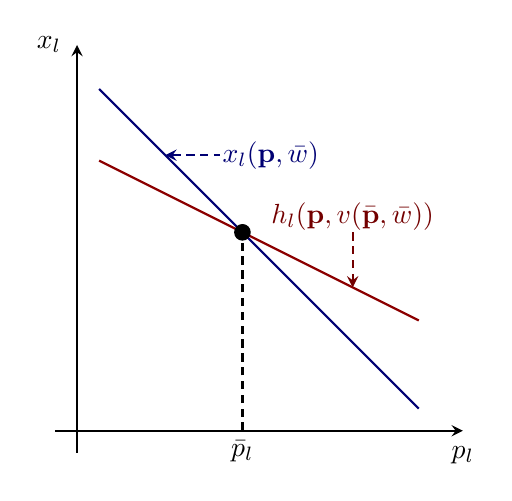
\begin{tikzpicture}[scale=1.4]
        % basics
        \draw [-stealth,color=black,thick] (-0.2,0) -- (3.5,0) node[below=2pt] {$p_l$};
        \draw [-stealth,color=black,thick] (0,-0.2) -- (0,3.5) node[left=2pt] {$x_l$};
        
        % walrasian
        \draw[domain=0.2:3.1, blue!45!black, thick, variable=\x] plot ({\x}, {3.3-\x});
        % hicksian
        \draw[domain=0.2:3.1, red!55!black, thick, variable=\x] plot ({\x}, {2.55-0.5*\x});
        % intersection: \bar{p}
        \filldraw[black] (1.5,1.8) circle (2pt); 
        % label
        \draw[densely dashed, thick, black] (1.5,0) node[below=0pt] {$\bar{p}_l$} (1.5,0) -- (1.5,1.8);
        
        % text
        \draw[-stealth,thick,densely dashed,red!45!black] (2.5,1.8) -- node[above=7pt] {$h_l(\mathbf{p},v(\bar{\mathbf{p}},\bar{w}))$} (2.5,1.3); % walrasian
        \draw[stealth-,thick,densely dashed,blue!45!black] (0.8,2.5) -- node[right=7pt] {$x_l(\mathbf{p},\bar{w})$} (1.3,2.5); % walrasian
    \end{tikzpicture}
    \caption*{Normal good}
\end{minipage}
\hfill
\begin{minipage}[b]{0.45\textwidth}
    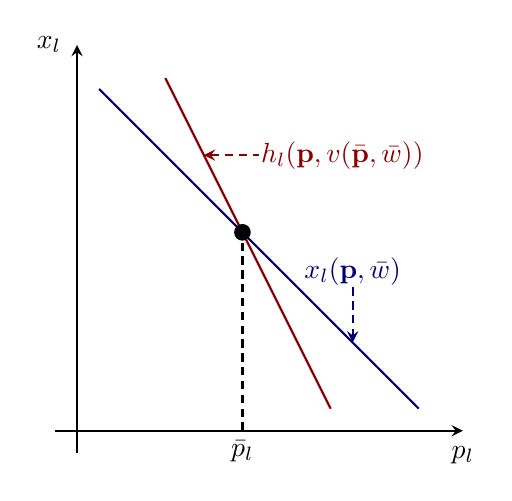
\begin{tikzpicture}[scale=1.4]
        % basics
        \draw [-stealth,color=black,thick] (-0.2,0) -- (3.5,0) node[below=2pt] {$p_l$};
        \draw [-stealth,color=black,thick] (0,-0.2) -- (0,3.5) node[left=2pt] {$x_l$};
        
        % walrasian
        \draw[domain=0.2:3.1, blue!45!black, thick, variable=\x] plot ({\x}, {3.3-\x});
        % hicksian
        \draw[domain=0.8:2.3, red!55!black, thick, variable=\x] plot ({\x}, {4.8-2*\x});
        % intersection: \bar{p}
        \filldraw[black] (1.5,1.8) circle (2pt); 
        % label
        \draw[densely dashed, thick, black] (1.5,0) node[below=0pt] {$\bar{p}_l$} (1.5,0) -- (1.5,1.8);
        
        % text
        \draw[-stealth,thick,densely dashed,blue!45!black] (2.5,1.3) -- node[above=7pt] {$x_l(\mathbf{p},\bar{w})$} (2.5,0.8); % walrasian
        \draw[stealth-,thick,densely dashed,red!55!black] (1.15,2.5) -- node[right=7pt] {$h_l(\mathbf{p},v(\bar{\mathbf{p}},\bar{w}))$} (1.65,2.5); % walrasian
    \end{tikzpicture}
    \caption*{Inferior good}
\end{minipage}
\end{figure}

When we focus on one good $l$, we have $\frac{\partial h_l(\bar{\mathbf{p}},\bar{u})}{\partial p_l} =\frac{\partial x_l(\bar{\mathbf{p}},\bar{w})}{\partial p_l} + \frac{\partial x_l (\bar{\mathbf{p}},\bar{w})}{\partial w}\cdot w_l(\bar{\mathbf{p}},\bar{w})$, the relationship between the Hicksian demand and the Walrasian demand becomes much more clear:
\begin{enumerate}
    \item[-] If good $l$ is normal good, then $\partial x_l (\bar{\mathbf{p}},\bar{w})/\partial w>0$, this means that if its price $p_l$ increases, Hicksian demand (with wealth increased accordingly to match the initial utility level $\bar{u}=v(\bar{\mathbf{p}},\bar{w})$) for good $l$ will decrease, but by a lower amount than the decrease of Walrasian demand (without wealth adjustment).
    \item[-] If good $l$ is inferior good, then $\partial x_l (\bar{\mathbf{p}},\bar{w})/\partial w<0$, the opposite logic follows. 
\end{enumerate}

Here, Slutsky (substitution) matrix appears once again. However, different from the choice-based, WARP-regulated demand, which requires the Slutsky matrix to be \textbf{negative semidefinite} and to satisfy $S(\mathbf{p},w)\mathbf{p}=0$ (see Thm.\ref{thm:slutksy_matrix_negativesemidef}), one extra condition is required for preference maximization: $S$ being \textbf{symmetric}.
The more essential distinction between these two approaches is that they adopt two different wealth compensation approaches: For an initial price-wealth pair $(\bar{\mathbf{p}},\bar{w})$ and its corresponding utility level $\bar{u}=u(\bar{x})$, and the price after change $\mathbf{p}'$:
\begin{enumerate}
    \item[-] Slutsky wealth compensation (Section\ref{chap2:sec2:ssec4}): wealth is adjusted from $\bar{w}$ to $w^S$ s.t. $\bar{x}$ could still be afforded, $w^S=\bar{x}\cdot \mathbf{p}'$, giving: $\Delta w_{\text{Slutsky}}=\mathbf{p}'\cdot x(\bar{\mathbf{p}},\bar{w})-\bar{w}$
    \item[-] Hicksian wealth compensation (this section): wealth is adjusted from from $\bar{w}$ to $w^H$ s.t. $\bar{u}$ could still be achieved, $v(\mathbf{p}',w^H)=\bar{u}$, giving: $\Delta w_{\text{Hicks}}=e(\mathbf{p}',\bar{u})-\bar{w}$
\end{enumerate}
The two compensation approaches are closely linked: $\Delta w_{\text{Hicks}}\leq \Delta w_{\text{Slutsky}}$, and since $\nabla_{\mathbf{p}}e(\bar{\mathbf{p}},\bar{u}) = h(\bar{\mathbf{p}},\bar{u})=x(\bar{\mathbf{p}},\bar{w})$, the equality holds \textbf{only} when the price change is a differential change ($\mathrm{d}p$):
\begin{align*}
    \Delta w_{\text{Slutsky}} &= \mathbf{p}'\cdot x(\bar{\mathbf{p}},\bar{w})-\bar{w} \\
    & \mathbf{p}'\cdot x(\bar{\mathbf{p}},\bar{w})-\bar{\mathbf{p}}\cdot x(\bar{\mathbf{p}},\bar{w})= x(\bar{\mathbf{p}},\bar{w})\cdot(\mathbf{p}'-\bar{\mathbf{p}}) \\
    & = \nabla_{\mathbf{p}}e(\bar{\mathbf{p}},\bar{u})\cdot(\mathbf{p}'-\bar{\mathbf{p}}) = e(\mathbf{p}',\bar{u})-e(\bar{\mathbf{p}},\bar{u})\\
    & = e(\mathbf{p}',\bar{u})-\bar{w} = \Delta w_{\text{Hicks}}
\end{align*}
the intuition is, for a very small change of price for good $l$, the total effect on the expenditure required to still achieve $\bar{u}$ is just the direct effect of the price change. But if the price change is not sufficiently small (discrete price changes), we would always have $\Delta w_{\text{Hicks}}< \Delta w_{\text{Slutsky}}$ (see Fig.\ref{fig:hicksian_slutsky_comp}).

\begin{figure}[ht]
    \centering
    \caption{Hicksian and Slutsky wealth compensation}
    \label{fig:hicksian_slutsky_comp}
    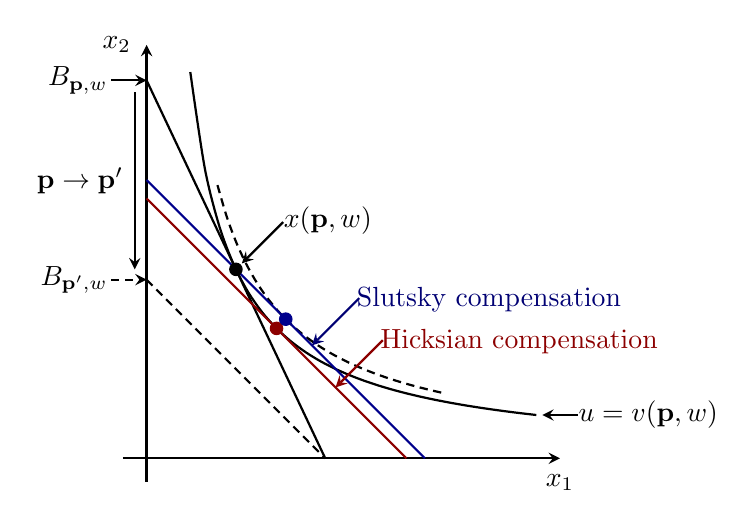
\begin{tikzpicture}[scale=1.5]
        % basics
        \draw [-stealth,color=black,thick] (-0.2,0) -- (3.5,0) node[below=2pt] {$x_1$};
        \draw [-stealth,color=black,thick] (0,-0.2) -- (0,3.5) node[left=2pt] {$x_2$};
        
        % utility and budget lines
        \draw[domain=0.37:3.3, smooth, thick, black, variable=\x] plot ({\x}, {1.1^2/\x}); % utility
        \draw[domain=0.6:2.5, smooth, thick, black, densely dashed, variable=\x] plot ({\x}, {(0.75625/2+1.1^2/(2*0.75625))^2/\x}); % slutsky utility
        \draw[domain=0:(4*1.1^2)/3.2, black, thick, variable=\x] plot ({\x}, {3.2-(3.2^2/(4*1.1^2))*\x}); % initial budget
        \draw[domain=0:(4*1.1^2)/3.2, densely dashed, black, thick, variable=\x] plot ({\x}, {(4*1.1^2)/3.2-\x}); % wealth-constant budget
        \draw[domain=0:2.2, red!55!black, thick, variable=\x] plot ({\x}, {2.2-\x}); % hicksian compensated budget
        \draw[domain=0:0.75625+1.1^2/0.75625, blue!55!black, thick, variable=\x] plot ({\x}, {0.75625+1.1^2/0.75625-\x}); % slutsky compensated budget
        
        % bundles
        \filldraw[black] (0.75625,1.1^2/0.75625) circle (1.5pt); % initial bundle
        \filldraw[red!55!black] (1.1,1.1) circle (1.5pt); % hicksian compensated bundle
        \filldraw[blue!55!black] (1.178125,1.178125) circle (1.5pt); % slutsky compensated bundle
        
        % texts and notes
        %% budget change
        \draw[-stealth,thick,black] (-0.3,3.2) -- node[left=4pt] {$B_{\mathbf{p},w}$} (0,3.2);
        
        \draw[-stealth,thick,densely dashed,black] (-0.3,1.5125) -- node[left=4pt] {$B_{\mathbf{p}',w}$} (0,1.5125);
        
        \draw[-stealth,thick] (-0.1,3.1) -- node[left=0.5pt] {$\mathbf{p}\rightarrow\mathbf{p}'$} (-0.1,1.6);
        
        %% utility
        \draw[stealth-,thick] (3.35,1.1^2/3.3) -- node[right=3pt] {$u=v(\mathbf{p},w)$} (3.65,1.1^2/3.3);
        
        
        %% bundles
        %%% initial bundle
        \draw[stealth-,thick,black] (0.75625+0.05,1.1^2/0.75625+0.05) -- node[right=4pt,yshift=8pt] {$x(\mathbf{p},w)$} (0.75625+0.4,1.1^2/0.75625+0.4);
        
        %%% Hicksian
        \draw[stealth-,thick,red!55!black] (1.6,0.6) -- node[right=4pt,yshift=8pt] {Hicksian compensation} (2,1);
         %%% Slutsky
        \draw[stealth-,thick,blue!45!black] (1.4,0.95625) -- node[right=4pt,yshift=8pt] {Slutsky compensation} (1.8,1.35625);
        
    \end{tikzpicture}
\end{figure}

\subsubsection*{$x(\mathbf{p},w)$ and $v(\mathbf{p},w)$}
Mirroring Thm.\ref{thm:hdemand_and_exp}, we can link the Walrasian demand $x(\mathbf{p},w)$ and indirect utility function $v(\mathbf{p},w)$ through \textbf{Roy's identity}:
\begin{theorem}{Roy's identity}{roy_identity}
    With a continuous $u(\cdot)$ representing a locally nonsatiated and strictly convex $\succsim$, and an indirect utility function differentiable at $(\bar{\mathbf{p}},\bar{w})\gg 0$, the \myhl[blue]{Walrasian demand $x(\mathbf{p},w)$} is the (negative) derivative vector of $v(\mathbf{p},w)$ w.r.t. prices $\mathbf{p}$, \textbf{normalized} by marginal indirect utility of wealth:
    $$x(\bar{\mathbf{p}},\bar{w})=-\frac{1}{\nabla_w v(\bar{\mathbf{p}},\bar{w})}\nabla_{\mathbf{p}}v(\bar{\mathbf{p}},\bar{w})$$
    that is, $x_l(\bar{\mathbf{p}},\bar{w})=- \frac{\partial v(\bar{\mathbf{p}},\bar{w})/\partial p_l}{\partial v(\bar{\mathbf{p}},\bar{w})/\partial w},\forall l=1,\cdots,L$
\end{theorem}

Again, Roy's identity will be proved with 3 different approaches:
\begin{enumerate}
    \item[\textit{\textbf{Proof 1}}]: Let $\bar{u} = v(\bar{\mathbf{p}},\bar{w})$. Since $v(\mathbf{p},e(\mathbf{p},\bar{u}))=\bar{u},\forall \mathbf{p}$, differentiate the equation w.r.t. $\mathbf{p}$ and evaluating at $\mathbf{p}=\bar{\mathbf{p}}$, get
    \begin{align*}
        & \nabla_{\mathbf{p}} v(\bar{\mathbf{p}},e(\bar{\mathbf{p}},\bar{u})) + \frac{\partial v(\bar{\mathbf{p}},e(\bar{\mathbf{p}},\bar{u}))}{\partial w} \nabla_{\mathbf{p}}e(\bar{\mathbf{p}},\bar{u})=0 \\
        \xRightarrow{\text{Thm.\ref{thm:hdemand_and_exp}}} & \nabla_{\mathbf{p}} v(\bar{\mathbf{p}},e(\bar{\mathbf{p}},\bar{u})) + \frac{\partial v(\bar{\mathbf{p}},e(\bar{\mathbf{p}},\bar{u}))}{\partial w} h(\bar{\mathbf{p}},\bar{u})=0\\
        \xRightarrow[\bar{w}=e(\bar{\mathbf{p}},\bar{u})]{h(\bar{\mathbf{p}},\bar{u})=x(\bar{\mathbf{p}},\bar{w})} & \nabla_{\mathbf{p}} v(\bar{\mathbf{p}},\bar{w}) + \frac{\partial v(\bar{\mathbf{p}},\bar{w})}{\partial w} x(\bar{\mathbf{p}},\bar{w})=0\\
        \Rightarrow & x(\bar{\mathbf{p}},\bar{w})=-\frac{1}{\nabla_w v(\bar{\mathbf{p}},\bar{w})}\nabla_{\mathbf{p}}v(\bar{\mathbf{p}},\bar{w})
    \end{align*}

    \item[\textit{\textbf{Proof 2}}] FOC argument: assume $x(\mathbf{p},w)\gg 0$ and differentiable at $(\bar(\mathbf{p}),\bar{u})$, then by the chain rule, we have 
    \begin{align*}
        \left. \frac{\partial v(\mathbf{p},w)}{\partial p_l} \right\vert_{(\bar{\mathbf{p}},\bar{w})}&=\sum^L_{k=1} \underbrace{\frac{\partial u\left(x(\bar{\mathbf{p}},\bar{w})\right)}{\partial x_k}}_{\equiv \lambda p_k \text{ (Lagrange)}} \frac{\partial x_k(\bar{\mathbf{p}},\bar{w})}{\partial p_l}\\
        &= \underbrace{\lambda}_{=\frac{\partial v(\bar{\mathbf{p}},\bar{w})}{\partial w}} \underbrace{\sum^L_{k=1}p_k \frac{\partial x_k(\bar{\mathbf{p}},\bar{w})}{\partial p_l}}_{\text{by Thm.\ref{thm:walraslaw_waldemand_thm2} }=-x_l(\bar{\mathbf{p}},\bar{w})}\\
        & = -\frac{\partial v(\bar{\mathbf{p}},\bar{w})}{\partial w} \cdot x_l(\bar{\mathbf{p}},\bar{w})\\
        \Rightarrow x_l(\bar{\mathbf{p}},\bar{w}) &= -\frac{\partial v(\bar{\mathbf{p}},\bar{w})/\partial p_l}{\partial v(\bar{\mathbf{p}},\bar{w})/\partial w}
    \end{align*}
    \item[\textit{\textbf{Proof 3}}] Envelope Theorem argument: by the Envelope Theorem, we have $\partial v(\bar{\mathbf{p}},\bar{w})/\partial p_l$ $= -\lambda x_l(\bar{\mathbf{p}},\bar{w})$, and $\partial v(\bar{\mathbf{p}},\bar{w})/\partial w=\lambda$, combining the two equations yields the proposition.
\end{enumerate}

With Roy's identity, it will be much easier to compute Walrasian demand from indirect utility, one only need to take derivatives instead of solving the system of FOC equations.

In summary, the duality between UMP and EMP have been established, and the four objects are interlinked with each other through the aforementioned properties (see Fig.\ref{fig:duality_relations}).

\begin{figure}[ht]
    \centering
    \caption{Duality of UMP and EMP}
    \label{fig:duality_relations}
    \begin{tikzpicture}[scale=1]
        \node (UMP) at (0,6.5) {\color{blue!45!black}\textbf{UMP}};
        \node (EMP) at (10,6.5) {\color{red!55!black}\textbf{EMP}};
        \node (wal) at (0,5) [draw,color=blue!45!black,fill=blue!45!black] {\color{white}$x(\mathbf{p},w)$};
        \node (val) at (0,0) [draw,color=blue!45!black] {$v(\mathbf{p},w)$};
        \node (hic) at (10,5) [draw,color=red!55!black,fill=red!55!black] {\color{white}$h(\mathbf{p},u)$};
        \node (exp) at (10,0) [draw,color=red!55!black] {$e(\mathbf{p},u)$};
        
        % UMP and EMP
        \draw[-stealth,thick,color=blue!45!black] (UMP.5) to node[above] {\small \color{black}Duality (Thm.\ref{thm:EMP_vs_UMP})} (EMP.175);
        \draw[stealth-,thick,color=red!55!black] (UMP.-5) to (EMP.185);
        
        % walrasian and hicksian
        \draw[-stealth,thick,color=blue!45!black] (wal.5) to node[above] {\small $\frac{\partial h_l(\mathbf{p},u)}{\partial p_k} = \frac{\partial x_l(\mathbf{p},w)}{\partial p_k} +\frac{\partial x_l(\mathbf{p},w)}{\partial w}x_k(\mathbf{p},w)$} (hic.175);
        
        \draw[stealth-stealth,thick,color=blue!45!black] (wal.260) to node[above,rotate=90] {\small $x(\mathbf{p},w)=-\frac{\nabla_{\mathbf{p}}v(\mathbf{p},w)}{\nabla_w v(\mathbf{p},w)}$} (val.100);
        
        \draw[stealth-stealth,thick,color=red!55!black] (hic.280) to node[above,rotate=270] {$h(\mathbf{p},u)=\nabla_{\mathbf{p}}e(\mathbf{p},u)$} (exp.80);
        
        \draw[-stealth,thick,color=blue!45!black] (val.5) to node[above] {\small $u=v(\mathbf{p},e(\mathbf{p},u))$} (exp.175);
        \draw[stealth-,thick,color=red!55!black] (val.-5) to node[below] {\small $w=e(\mathbf{p},v(\mathbf{p},w)$} (exp.185);
        
        \draw[-stealth-=.4,thick,color=red!55!black] (hic.260) to (val.80);
        \draw[-stealth,thick,color=blue!45!black] (val.80) to node[above,rotate=-90] {\small $x(\mathbf{p},w)=h(\mathbf{p},v(\mathbf{p},w))$} (wal.280);
        
        \draw[-stealth-=.4,thick,color=blue!45!black] (wal.280) to (exp.100);
        \draw[-stealth,thick,color=red!55!black] (exp.100) to node[above,rotate=90] {\small $h(\mathbf{p},u)=x(\mathbf{p},e(\mathbf{p},u))$} (hic.260);
    \end{tikzpicture}
\end{figure}

Empirically, Walrasian demand $x(\mathbf{p},w)$ can be observed (in principle), or relatively easily computed from the indirect utility $v(\mathbf{p},w)$ via Roy's Identity; Hicksian demand $h(\mathbf{p},u)$ can be derivated from the observable $x(\mathbf{p},w)$ through the Slutsky equation, and the expenditure function $e(\mathbf{p},u)$ can be derived from $h(\mathbf{p},u)$ by integration w.r.t. prices. 
Therefore, all objects of interest in the preference-based consumer theory can indeede be inferred (or justified) by a rational preference.